\documentclass[
	a4paper,
	12pt,
	% --- Opções da classe ---
	% Oneside para impressão apenas no verso. Opção twoside para impressão frente e verso.
	oneside,
	% --- Estilo de citação ---
	% Opções do pacote abntex2cite:
	% -- Citação por nome e ano
	alf,
	% -- Formato das referências justificado na margem
	bibjustif
]{tex/config/monografia}

% --- PACOTES ---
\usepackage[portuguese]{babel}
\usepackage[utf8]{inputenc}
\usepackage{graphicx} % Para incluir figuras
\usepackage{lipsum} % Apenas para texto de exemplo, pode remover depois
\usepackage{setspace} % Para controle de espaçamento (doublespacing, etc.)
\usepackage{amsmath} % Para comandos matemáticos como \text{}
\usepackage{booktabs} % Para tabelas com \toprule, \midrule, \bottomrule
\usepackage{subcaption} % Para o ambiente subfigure
\usepackage[alf,abnt-repeated-title-omit=yes,bibjustif]{abntex2cite} % Carrega o pacote de citações

\graphicspath{{figuras/}} % Diz ao LaTeX para procurar imagens nesta pasta


% --- DEFINIÇÕES DO DOCUMENTO (Informações do TCC) ---
% (Movido de pretexto.tex para cá para centralizar a configuração)

% --- Título e Autor ---
\titulo{Modelo baseado em Attention-LSTM para previsão de concentração de PM2.5}
\autor{Daniel Fagundes Portes Fernandes}
\nome{Daniel}
\ultimonome{Fernandes}

% --- Curso e Grau ---
\bacharelado
\curso{Ciência da Computação}
\dia{02} \mes{dezembro} \ano{2023}
\cidade{Juiz de Fora}

% --- Instituição ---
\instituicao{Universidade Federal de Juiz de Fora} \sigla{UFJF}
\unidadeacademica{INSTITUTO DE CIÊNCIAS EXATAS}
\departamento{DEPARTAMENTO DE CIÊNCIA DA COMPUTAÇÃO}

% --- Banca ---
\orientador{Luciana Conceição Dias Campos}
\ttorientador{Doutora em Engenharia Elétrica PUC-Rio}
\examinadorum{} % Deixa vazio se não tiver
\ttexaminadorum{} % Deixa vazio se não tiver
\examinadordois{} % Deixa vazio se não tiver
\ttexaminadordois{} % Deixa vazio se não tiver


\begin{document}

\maketitle

\begin{dedicatoria}
    Aos meus amigos e irmãos.

    Aos meus pais, pelo apoio e sustento.
\end{dedicatoria}
\agradecimento{Agradecimentos}
\indent A todos os meus parentes, pelo encorajamento e apoio.

Ao meu orientador, pela orientação, amizade e principalmente, pela paciência, sem a qual este trabalho não se realizaria.

Aos professores do Departamento de Ciência da Computação pelos seus ensinamentos e aos funcionários do curso, que durante esses anos, contribuíram de algum modo para o meu enriquecimento pessoal e profissional.
\begin{epigrafe}
``Lembra que o sono é sagrado e alimenta de horizontes o tempo acordado de viver.''

\hfill Beto Guedes (Amor de Índio)
\end{epigrafe}
\resumo{Resumo}
O material particulado fino (PM2,5) é um poluente atmosférico crítico, associado a agravos à saúde pública, sobrecarga de sistemas de saúde e impactos ambientais. A previsão horária de curto prazo é, portanto, uma ferramenta relevante para análise ambiental, apoio a alertas e gestão da qualidade do ar. Contudo, essa tarefa é desafiadora devido à natureza não linear, ruidosa e frequentemente incompleta das séries de monitoramento, além da dependência de variáveis meteorológicas, temporais e de emissão. Este trabalho propõe um estudo experimental comparativo para previsão horária de PM2,5 com horizonte de 24 horas na estação Sapo, pertencente ao recorte CMD (Conceição do Mato Dentro, MG) do conjunto de dados. A estação foi selecionada por combinar alta cobertura de PM2,5, presença pareada de PM10 e ocorrência suficiente de eventos de maior concentração para sustentar a comparação entre modelos. O protocolo utiliza as 48 horas antecedentes como janela de entrada e inclui variáveis preditoras derivadas de PM2,5, PM10, indicadores temporais, termos de Fourier para sazonalidade e substitutos causais de PM10 disponíveis no instante da previsão. Também foi aplicado mascaramento para excluir valores imputados do alvo da função de perda e das métricas de avaliação. Foram comparados modelos LSTM, arquiteturas Seq2Seq com e sem atenção e XGBoost multissaída como modelo de referência tabular, com ajuste de hiperparâmetros por validação temporal \textit{walk-forward} e análise de robustez por múltiplas sementes. Nos resultados principais, a LSTM direta destacou-se como o modelo mais equilibrado em erro médio. O XGBoost consolidou-se como modelo de referência tabular forte, enquanto o Seq2Seq com atenção melhorou parte do comportamento em picos sem superar a LSTM direta no erro médio. Experimentos diagnósticos com variáveis auxiliares futuras elevaram o \(R^2\), evidenciando que parte da variância horária depende de informações não disponíveis causalmente no cenário operacional. Conclui-se que a modelagem deve equilibrar minimização do erro médio, preservação da amplitude dos picos e disponibilidade causal de variáveis explicativas.

\noindent \ \textbf{Palavras-chave:} PM2,5, Previsão de Séries Temporais, Aprendizado Profundo, LSTM, Seq2Seq, XGBoost, Qualidade do Ar.

\resumo{Abstract}
Fine particulate matter (PM2.5) is a critical air pollutant associated with public health burdens and environmental impacts. Short-term hourly forecasting is therefore relevant for environmental analysis, warning support, and air-quality management. However, this task is challenging because monitoring series are nonlinear, noisy, often incomplete, and influenced by meteorological, temporal, and emission-related factors. This work proposes a comparative experimental study for 24-hour-ahead hourly PM2.5 forecasting at the Sapo station, within the CMD subset (Conceição do Mato Dentro, Minas Gerais, Brazil) of the dataset. The station was selected because it combines high PM2.5 coverage, paired PM10 availability, and enough higher-concentration events to support model comparison. The protocol uses the previous 48 hours as input and includes predictors derived from PM2.5, PM10, temporal indicators, Fourier seasonality terms, and causal PM10 proxies available at prediction time. Target masking is also applied to exclude imputed target values from the loss function and evaluation metrics. The study compares LSTM models, Seq2Seq architectures with and without attention, and multi-output XGBoost as a tabular reference model, using walk-forward hyperparameter tuning and multi-seed robustness analysis. In the main results, direct LSTM stood out as the most balanced model in terms of average error. XGBoost remained a strong tabular reference model, while attention-based Seq2Seq improved part of the peak behavior without surpassing direct LSTM in average error. Diagnostic experiments with future auxiliary variables increased \(R^2\), indicating that part of the hourly variance depends on information that is not causally available in the operational setting. The results show that forecasting design must balance average-error minimization, peak-amplitude preservation, and the causal availability of explanatory variables.

\noindent \ \textbf{Keywords:} PM2.5, Time Series Forecasting, Deep Learning, LSTM, Seq2Seq, XGBoost, Air Quality.

\tableofcontents \thispagestyle{empty}
\listoffigures \thispagestyle{empty}
\listoftables \thispagestyle{empty}

\chapter*{Lista de Abreviações}
\addcontentsline{toc}{chapter}{Lista de Abreviações}
\begingroup
\footnotesize
\renewcommand{\arraystretch}{0.86}
\setlength{\tabcolsep}{3pt}
\begin{tabular}{@{}p{0.18\textwidth}p{0.76\textwidth}@{}}
	ARIMA & Autoregressive Integrated Moving Average \\
	BRITS & Bidirectional Recurrent Imputation for Time Series \\
	CMD & Conceição do Mato Dentro \\
	CNN & Convolutional Neural Network (Rede Neural Convolucional) \\
	CNN-LSTM & Convolutional Neural Network combinada com Long Short-Term Memory \\
	CV & Cross-Validation (Validação Cruzada) \\
	DA-RNN & Dual-stage Attention-based Recurrent Neural Network \\
	EDA & Análise Exploratória de Dados \\
	ERA5 & Produto de reanálise atmosférica ERA5 \\
	FEAM & Fundação Estadual do Meio Ambiente \\
	GNSS & Global Navigation Satellite System \\
	GNSS-PWV & Precipitable Water Vapor estimado por GNSS \\
	HPO & Hyperparameter Optimization (Otimização de Hiperparâmetros) \\
	KNN & K-Nearest Neighbors \\
	LSTM & Long Short-Term Memory \\
	MAE & Mean Absolute Error (Erro Médio Absoluto) \\
	MAPE & Mean Absolute Percentage Error (Erro Percentual Médio Absoluto) \\
	MBE & Mean Bias Error (Erro Médio de Viés) \\
	MICE & Multivariate Imputation by Chained Equations \\
	NLP & Natural Language Processing (Processamento de Linguagem Natural) \\
	NRMSE & Normalized Root Mean Squared Error (RMSE normalizado) \\
	Peak35 MAE & MAE para PM2,5 \(\geq 35\) \\
	PM & Particulate Matter (material particulado) \\
	PM10 & Material particulado com diâmetro de até 10 micrômetros \\
	PM2,5 & Material particulado fino, com diâmetro de até 2,5 micrômetros \\
	PTS & Partículas Totais em Suspensão \\
	PWV & Precipitable Water Vapor (Vapor de Água Precipitável) \\
	\(R^2\) & Coeficiente de Determinação \\
	ReLU & Rectified Linear Unit \\
	RF & Random Forest \\
	RF-LSTM & Random Forest combinado com Long Short-Term Memory \\
	RMSE & Root Mean Squared Error (Raiz do Erro Quadrático Médio) \\
	RNN & Recurrent Neural Network (Rede Neural Recorrente) \\
	SAITS & Self-Attention-based Imputation for Time Series \\
	Seq2Seq & Sequence-to-Sequence \\
	SVM & Support Vector Machine (Máquina de Vetores de Suporte) \\
	TCC & Trabalho de Conclusão de Curso \\
	TF & Teacher Forcing \\
	TFT & Temporal Fusion Transformer \\
	TPE & Tree-structured Parzen Estimator \\
	UFJF & Universidade Federal de Juiz de Fora \\
	XGBoost & Extreme Gradient Boosting \\
\end{tabular}
\endgroup
\thispagestyle{empty}



% =========================================================================
% ELEMENTOS TEXTUAIS (SEUS CAPÍTULOS)
% =========================================================================
\pagestyle{ruledheader} % Estilo de cabeçalho para o corpo do texto
\pagenumbering{arabic} % Começa a contagem de páginas arábicas aqui

% cap_introducao.tex
\chapter{Introdução}
\label{chap:introducao}

A poluição atmosférica por material particulado fino (\textit{Particulate Matter}, PM2.5) permanece entre os problemas ambientais de maior impacto direto sobre a saúde pública. Por possuir diâmetro aerodinâmico inferior a 2,5 micrômetros, esse poluente consegue penetrar profundamente no sistema respiratório e está associado a desfechos respiratórios e cardiovasculares adversos \cite{who2021air,pope2006health,brook2010particulate}. A carga global de doença atribuível à poluição atmosférica por partículas finas reforça a importância de sistemas de monitoramento, prevenção e resposta \cite{cohen2017estimates}. No Brasil, episódios associados a queimadas e transporte atmosférico também ampliam a relevância do tema, com impactos mensuráveis sobre internações e mortalidade \cite{requia2021health,requia2022short}.

Nesse contexto, prever a concentração horária de PM2.5 com antecedência útil pode apoiar alertas, análise ambiental e planejamento operacional em regiões monitoradas. A previsão de curto prazo busca estimar valores futuros a partir de medições recentes e de variáveis auxiliares disponíveis no instante da previsão. Em uma formulação horária, o modelo deve reconhecer padrões de persistência, ciclos diários, mudanças graduais e eventos abruptos para produzir estimativas úteis para as próximas horas.

A tarefa, entretanto, é tecnicamente desafiadora. Séries ambientais reais combinam autocorrelação, sazonalidade, picos raros, mudanças de regime, ruído instrumental e lacunas de medição. Além disso, PM2.5 depende de condições atmosféricas, fontes de emissão, transporte de poluentes e relações com outros poluentes, nem sempre medidos de forma completa. Quando essas variáveis não estão disponíveis no momento da previsão, o modelo precisa operar com informação parcial, o que limita o desempenho possível mesmo com arquiteturas mais sofisticadas.

A literatura recente tem explorado modelos de aprendizado profundo para previsão de PM2.5, incluindo redes recorrentes, LSTM e arquiteturas com codificador, decodificador e atenção \cite{yang2023attention,zhao2021pm2,zhang2021deep}. Essas abordagens são atrativas porque conseguem modelar dependências temporais e relações não lineares. Ao mesmo tempo, revisões da área apontam dificuldade de comparação entre trabalhos, pois resultados dependem do conjunto de dados, horizonte de previsão, variáveis utilizadas e desenho de validação \cite{pm25_review_2024}. Em séries temporais, a separação cronológica e a avaliação fora da amostra também são parte central da validade experimental \cite{tashman2000out,bergmeir2012crossvalidation,hyndman2021forecasting}.

Este trabalho parte desse problema metodológico. Em vez de propor uma nova arquitetura como contribuição central, o TCC desenvolve um estudo experimental comparativo para previsão horária de PM2.5 na estação Sapo, pertencente ao recorte CMD (Conceição do Mato Dentro, MG) do conjunto de dados utilizado neste trabalho. A fonte bruta pertence ao monitoramento contínuo de qualidade do ar disponibilizado pela Fundação Estadual do Meio Ambiente de Minas Gerais \cite{feam2026dadosmonitoramento}. A escolha da estação é detalhada na metodologia, mas se apoia em três aspectos principais: cobertura do alvo PM2.5, disponibilidade pareada de PM10 e ocorrência suficiente de eventos de maior concentração.

\section{Motivação}

A motivação deste TCC é prática e metodológica. Do ponto de vista prático, previsões horárias de PM2.5 podem apoiar decisões de curto prazo em qualidade do ar, especialmente quando há risco de aumento de concentração nas próximas horas. Para isso, não basta obter uma métrica média aceitável: o modelo também precisa ser avaliado quanto à sua capacidade de preservar a amplitude de picos e de manter desempenho ao longo do horizonte de previsão.

Do ponto de vista metodológico, a comparação entre modelos só é informativa quando as decisões de dados e avaliação são controladas. Caso cada modelo use outro recorte temporal, outro conjunto de atributos, outra imputação ou outro teste, a comparação deixa de medir apenas a escolha de modelagem. Neste trabalho, um protocolo rastreável significa que a estação, o período, a tarefa, a preparação dos dados, os atributos disponíveis, a separação temporal e as métricas são explicitados e mantidos de forma comum sempre que possível. Assim, a análise busca responder não apenas qual modelo teve menor erro médio, mas também quais decisões explicam ganhos, falhas e compromissos observados.

A formulação principal usa uma janela de 48 horas passadas para prever as próximas 24 horas. Essa escolha é motivada por uma necessidade operacional de previsão do dia seguinte e pela presença de padrões diários em séries horárias de qualidade do ar. As 48 horas antecedentes permitem ao modelo observar dois ciclos diários recentes, enquanto o horizonte de 24 horas preserva uma tarefa de curto prazo suficientemente exigente para comparar degradação por horizonte. A justificativa empírica e os detalhes do protocolo são apresentados nos capítulos de fundamentação e metodologia.

\section{Problema de Pesquisa}

Para investigar o problema, o estudo compara modelos sequenciais e um modelo de referência tabular sob a mesma preparação de dados e o mesmo período cronológico de teste reservado. Esse modelo de referência é o XGBoost com saída múltipla, usado como comparação forte não sequencial para que os ganhos dos modelos recorrentes e Seq2Seq sejam interpretados com cautela.

A pergunta central deste trabalho pode ser formulada da seguinte forma:

\begin{quote}
Em uma tarefa horária de previsão de PM2.5 na estação Sapo, como diferentes escolhas de modelagem e preparação dos dados afetam o erro médio, os erros por horizonte e a capacidade de representar eventos de maior concentração?
\end{quote}

\section{Objetivos}

\subsection{Objetivo Geral}

Avaliar, sob um protocolo experimental rastreável e comparável, o desempenho de modelos de aprendizado de máquina e aprendizado profundo para previsão horária de múltiplos passos de PM2.5 na estação Sapo, distinguindo erro médio global, erros por horizonte e capacidade de representar regimes de maior concentração.

\subsection{Objetivos Específicos}

\begin{enumerate}
    \item Definir um protocolo rastreável de previsão horária de PM2.5 para a estação Sapo, com tarefa de múltiplos passos, entrada de 48 horas e horizonte de 24 horas.
    \item Consolidar uma base de dados com PM2.5, PM10, variáveis temporais, variáveis exógenas causalmente disponíveis, imputação controlada, normalização e exclusão de valores imputados do alvo na perda e nas métricas.
    \item Comparar LSTM, Seq2Seq e XGBoost multissaída, usando o XGBoost como modelo de referência tabular forte sob a mesma preparação de dados e o mesmo período cronológico de teste.
    \item Avaliar os resultados por métricas globais, métricas por horizonte e comportamento em picos/cauda, separando erro médio de capacidade de representar eventos de maior concentração.
    \item Documentar resultados negativos, limitações e compromissos de modelagem, especialmente no uso de atenção, perdas ponderadas, variáveis exógenas e estratégias voltadas a picos.
\end{enumerate}

\section{Organização do Trabalho}

Este documento está estruturado em seis capítulos. O Capítulo \ref{chap:introducao} apresenta o contexto, a motivação, o problema de pesquisa e os objetivos. O Capítulo \ref{chap:fundamentacao_teorica} reúne os conceitos necessários para fundamentar o trabalho, incluindo PM2.5, séries temporais, dados faltantes, modelos recorrentes, Seq2Seq, atenção, XGBoost e métricas de avaliação. O Capítulo \ref{chap:trabalhos_relacionados} posiciona o trabalho na literatura de previsão de qualidade do ar e discute lacunas de comparabilidade experimental. O Capítulo \ref{chap:materiais_metodos} descreve a metodologia do trabalho, incluindo dados, protocolo experimental, modelos, treinamento e métricas. O Capítulo \ref{chap:resultados} apresenta os resultados principais e as análises dos experimentos realizados. Por fim, o Capítulo \ref{chap:conclusao} sintetiza as conclusões, limitações e possibilidades de continuidade.

% cap_fundamentacao.tex
\chapter{Fundamentação Teórica}
\label{chap:fundamentacao_teorica}

Este capítulo apresenta os conceitos teóricos necessários para fundamentar a previsão horária multi-horizonte de material particulado fino (PM2,5) em séries temporais ambientais. O foco recai sobre dados faltantes, variáveis exógenas conhecidas no momento da previsão, redes neurais artificiais, modelos recorrentes, arquiteturas codificador-decodificador com atenção e modelos baseados em árvores com impulsionamento por gradiente (\textit{gradient boosting}).

\section{Material Particulado Fino (PM2,5) e Monitoramento da Qualidade do Ar}

O material particulado fino (PM2,5) é formado por partículas com diâmetro aerodinâmico de até 2,5 micrômetros. O diâmetro aerodinâmico é uma forma de expressar o comportamento da partícula no ar: partículas menores permanecem suspensas por mais tempo e podem ser inaladas com maior facilidade. Por seu tamanho reduzido, o PM2,5 pode atingir regiões profundas do sistema respiratório e está associado a efeitos respiratórios e cardiovasculares relevantes \cite{pope2006health,brook2010particulate}. As diretrizes globais da Organização Mundial da Saúde tratam PM2,5 e material particulado com diâmetro aerodinâmico de até 10 micrômetros (PM10) como poluentes prioritários para avaliação de qualidade do ar \cite{who2021air}.

PM10, por sua vez, representa partículas com diâmetro aerodinâmico de até 10 micrômetros. Embora seja uma fração mais grossa que PM2,5, sua concentração pode carregar informação sobre condições ambientais, emissão de partículas e episódios de maior concentração. Por isso, em problemas de previsão, PM10 pode ser usado como variável auxiliar quando está disponível de forma compatível com a série de PM2,5.

Em redes de monitoramento, sensores registram concentrações de poluentes em intervalos regulares e formam séries temporais. Uma série temporal de qualidade do ar, portanto, é uma sequência de medições ordenadas pelo tempo. A previsão de curto prazo busca estimar concentrações futuras a partir de medições recentes e de informações auxiliares conhecidas no momento da previsão. Em formulações horárias, é comum usar um bloco de observações passadas para prever um ou mais instantes futuros.

\section{Séries Temporais Multivariadas}

Uma série temporal é uma sequência de observações indexadas no tempo. Em qualidade do ar, a concentração de um poluente depende de autocorrelação, ciclos diários e semanais, condições meteorológicas, variações de emissão, mudanças de regime e eventos raros. Quando múltiplas variáveis são observadas simultaneamente, como PM2,5, PM10 e atributos de calendário, a tarefa passa a ser multivariada. Nesse caso, o modelo não observa apenas o histórico do alvo, mas também outras informações que podem ajudar a explicar sua variação.

A análise de séries temporais costuma separar padrões em componentes interpretáveis. \citeonline{hyndman2021forecasting} distinguem tendência, sazonalidade, ciclos e variações remanescentes como padrões úteis para escolher métodos de previsão. Em uma decomposição aditiva simples, uma observação pode ser representada por:

\[
    y_t = T_t + S_t + R_t,
\]

em que \(T_t\) representa tendência ou tendência-ciclo, \(S_t\) representa sazonalidade de período conhecido e \(R_t\) representa o restante da série, incluindo ruído, mudanças abruptas e eventos raros. Para séries horárias, pode haver mais de uma sazonalidade relevante, como ciclo diário, semanal e anual. Essa leitura fundamenta o uso de atributos temporais, termos periódicos e defasagens como formas de representar dependências temporais sem recorrer a informação futura.

Outro conceito central é autocorrelação, isto é, a associação entre a série e versões defasadas dela mesma. Para uma defasagem \(\ell\), a autocorrelação amostral pode ser escrita como:

\[
    \rho(\ell)=
    \frac{
        \sum_t (y_t-\bar{y})(y_{t-\ell}-\bar{y})
    }{
        \sum_t (y_t-\bar{y})^2
    }.
\]

Valores altos de \(\rho(1)\), \(\rho(24)\) ou \(\rho(168)\) indicam, respectivamente, persistência de curto prazo, repetição diária e repetição semanal. Em problemas de previsão, essa leitura ajuda a escolher janelas históricas, defasagens sazonais e termos cíclicos adequados ao período de amostragem da série.

Formalmente, seja $\mathbf{x}_t \in \mathbb{R}^{d}$ o vetor de atributos observado no instante $t$, $y_t \in \mathbb{R}$ a concentração de PM2,5 e $\mathbf{z}_{t+k}$ o vetor de atributos futuros conhecidos no instante de emissão da previsão, como calendário, termos periódicos ou previsões meteorológicas disponíveis operacionalmente. Uma janela de entrada é o bloco de valores passados entregue ao modelo; o horizonte é o conjunto de instantes futuros que se deseja prever. Para uma janela de entrada de tamanho $L$ e horizonte $H$, o problema pode ser escrito como:

\[
    \hat{\mathbf{y}}_{t+1:t+H}
    =
    f_{\theta}\left(
        \mathbf{x}_{t-L+1:t},
        \mathbf{z}_{t+1:t+H}
    \right),
\]

em que $f_{\theta}$ é o modelo treinado e $\hat{\mathbf{y}}_{t+1:t+H} = (\hat{y}_{t+1}, \ldots, \hat{y}_{t+H})$. Essa formulação explicita a diferença entre variáveis observadas apenas no passado e variáveis conhecidas para o horizonte futuro.

Em problemas de previsão, a ordem temporal dos dados deve ser preservada. Separações aleatórias, comuns em tarefas com registros independentes, podem introduzir vazamento de informação futura em séries temporais. Por isso, avaliações fora da amostra e divisões cronológicas são recomendadas para estimar desempenho em um cenário próximo ao uso real \cite{hyndman2021forecasting,tashman2000out,bergmeir2012crossvalidation}.

\subsection{Validação cruzada temporal e \textit{walk-forward}}

A validação cruzada tradicional divide os dados em partições e assume exemplos aproximadamente independentes. Essa suposição não vale diretamente para séries temporais, nas quais observações vizinhas compartilham autocorrelação, sazonalidade e tendência. Em previsão, uma avaliação coerente deve respeitar a direção do tempo: o modelo só pode ser treinado com dados anteriores ao período validado. Essa preocupação é central em testes fora da amostra para previsão \cite{tashman2000out} e motiva adaptações da validação cruzada para séries temporais \cite{bergmeir2012crossvalidation,hyndman2021forecasting}.

Uma adaptação comum é a validação cruzada temporal por janela expansiva, também chamada de \textit{walk-forward validation}. Nesse procedimento, cada partição usa uma janela de treino que termina antes do bloco de validação seguinte. A cada nova partição, a janela de treino se expande e a validação avança para um período futuro. Assim, a avaliação considera várias origens temporais de previsão sem permitir que dados futuros influenciem o treinamento. Para \(K\) partições, a métrica de seleção pode ser resumida pela média:

\[
    \mathcal{L}_{CV}
    =
    \frac{1}{K}\sum_{k=1}^{K}
    \mathcal{L}_{val}^{(k)}.
\]

O subscrito \(CV\) indica \textit{cross-validation}, isto é, validação cruzada. Em desenhos experimentais com seleção de hiperparâmetros, a validação cruzada temporal pode ser aplicada dentro de um bloco de desenvolvimento. Ela não substitui uma avaliação cronológica final separada: esse conjunto permanece reservado para estimar o desempenho fora da amostra depois da seleção. A Figura~\ref{fig:validacao_cruzada_temporal_walk_forward} ilustra uma janela expansiva com três partições e avaliação final reservada.

\begin{figure}[htbp]
    \centering
    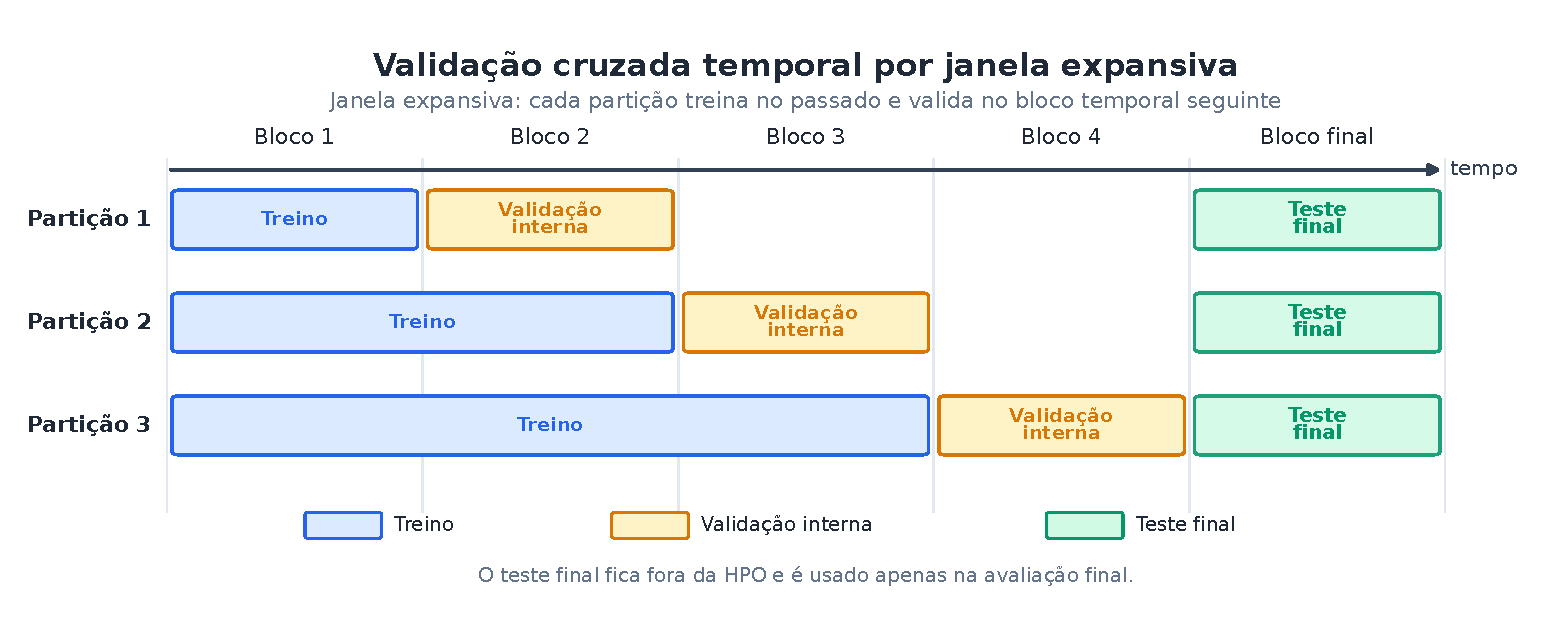
\includegraphics[width=\linewidth]{validacao_cruzada_temporal_walk_forward.pdf}
    \caption[Validação cruzada temporal por janela expansiva]{Validação cruzada temporal por janela expansiva, ou \textit{walk-forward validation}. Cada partição treina com dados passados e valida no bloco temporal seguinte; a avaliação final permanece reservada para estimar desempenho fora da amostra. Elaboração própria com base em \citeonline{tashman2000out}, \citeonline{bergmeir2012crossvalidation} e \citeonline{hyndman2021forecasting}.}
    \label{fig:validacao_cruzada_temporal_walk_forward}
\end{figure}

\section{Previsão Multi-Horizonte}

Na previsão multi-horizonte, o objetivo é estimar mais de um instante futuro. Para uma entrada $\mathbf{x}_{t-L+1:t}$ e um horizonte de \(H\) instantes, o modelo deve produzir $\hat{\mathbf{y}}_{t+1:t+H}$. Revisões recentes de previsão com aprendizado profundo descrevem arquiteturas de codificador e decodificador tanto para previsão de horizonte único quanto para previsão multi-horizonte \cite{lim2021survey,benidis2022deep}. Três estratégias são especialmente relevantes:

\begin{itemize}
    \item \textbf{Previsão recursiva:} o modelo aprende uma função de horizonte único $\hat{y}_{t+1}=g_{\theta}(\mathbf{x}_{t-L+1:t})$ e realimenta suas próprias saídas para obter $\hat{y}_{t+2}, \ldots, \hat{y}_{t+H}$. A estratégia é simples, mas pode acumular erros ao longo do horizonte.
    \item \textbf{Previsão direta:} o modelo aprende diretamente $\hat{\mathbf{y}}_{t+1:t+H}=g_{\theta}(\mathbf{x}_{t-L+1:t})$. Isso reduz a realimentação de erro, mas exige aprender a estrutura conjunta do horizonte.
    \item \textbf{Codificador-decodificador:} uma rede codifica a janela de entrada e outra gera a sequência futura, possivelmente condicionada por variáveis conhecidas no horizonte. Essa formulação é natural para tarefas sequência-para-sequência.
\end{itemize}

Essas alternativas podem ser implementadas com modelos recorrentes, arquiteturas codificador-decodificador e modelos baseados em árvores com saída múltipla. Comparações desse tipo são necessárias porque a literatura de previsão não sustenta uma única arquitetura universalmente dominante; revisões de redes neurais recorrentes para séries temporais ressaltam que não existem soluções universais em previsão \cite{hewamalage2021rnn}.

\section{Dados Faltantes, Imputação e Vazamento Temporal}

Dados ambientais reais frequentemente contêm lacunas por falhas de sensor, manutenção, comunicação ou filtragem de leituras inconsistentes. Uma lacuna significa que, em determinado instante, a medição esperada não foi observada. A ausência de dados deve ser tratada com cuidado porque pode afetar tanto o treinamento quanto a avaliação. A literatura de dados faltantes diferencia o valor não observado do valor realmente medido; tratá-los como equivalentes pode distorcer inferências e métricas \cite{rubin1976inference}.

Imputação é o processo de preencher lacunas com estimativas. Métodos simples, como interpolação linear, preservam a estrutura temporal local e são transparentes; métodos multivariados, como Multivariate Imputation by Chained Equations (MICE) e MissForest, exploram relações entre variáveis \cite{vanbuuren2011mice,stekhoven2012missforest}. Métodos de imputação temporal, como Bidirectional Recurrent Imputation for Time Series (BRITS) e Self-Attention-based Imputation for Time Series (SAITS), também usam máscaras de observação para distinguir valores disponíveis de valores ausentes \cite{cao2018brits,du2023saits}. Neste contexto, máscara significa um indicador que informa se um valor foi originalmente observado ou se foi preenchido por algum método de imputação. Independentemente do método escolhido, essa distinção é importante: valores preenchidos não devem ser tratados automaticamente como observações reais. Por isso, protocolos de previsão com lacunas precisam preservar informação sobre ausência e explicitar como a imputação afeta treinamento e avaliação.

Outro risco é o vazamento temporal. A imputação, a normalização e a criação de atributos precisam ser ajustadas sem usar estatísticas futuras indisponíveis no instante de previsão. Em um protocolo cronológico, esses procedimentos devem ser definidos com informação anterior ao período avaliado.

\section{Janelas e Variáveis Exógenas}

Modelos supervisionados de séries temporais costumam converter uma sequência contínua em pares de entrada e saída por janelas deslizantes. Cada amostra é formada por uma janela histórica de \(L\) instantes e por um alvo futuro com \(H\) instantes. Em termos simples, o modelo recebe um trecho do passado e aprende a produzir um trecho do futuro. A sobreposição entre janelas aumenta o número de exemplos, mas exige cuidado para manter a divisão temporal e evitar que uma janela de treino alcance o período de validação ou teste.

Defasagens explícitas e variáveis exógenas podem aumentar a informação disponível para o modelo. Defasagem é o uso de valores passados de uma variável, como a concentração observada uma hora ou vinte e quatro horas antes. Variável exógena é uma informação externa ao alvo principal, como PM10, temperatura, vento ou atributos de calendário. No entanto, uma variável exógena só pode entrar no decodificador se estiver disponível no momento em que a previsão seria feita. Atributos de calendário, termos periódicos e previsões meteorológicas publicadas antes da emissão da previsão são exemplos de informação potencialmente disponível. Já variáveis observadas apenas no futuro, como medições futuras de outro poluente, não devem ser usadas diretamente.

\section{Redes Neurais e Aprendizado Profundo}
\label{sec:redes_neurais_deep_learning}

Redes neurais artificiais são modelos paramétricos compostos por unidades simples conectadas por pesos. A inspiração histórica vem de modelos computacionais do neurônio biológico, como o neurônio lógico de \citeonline{mcculloch1943logical} e o perceptron de \citeonline{rosenblatt1958perceptron}. Essa relação, porém, deve ser entendida como uma analogia didática. Redes neurais usadas em aprendizado de máquina não simulam de forma completa a fisiologia de neurônios reais; elas usam uma abstração matemática capaz de combinar entradas, ajustar pesos e produzir saídas.

Em um neurônio biológico, dendritos recebem sinais, o corpo celular integra parte dessas informações e o axônio transmite sinais para outras células. Em um neurônio artificial, a operação análoga é representada por entradas numéricas, pesos, viés e uma função de ativação. A Figura~\ref{fig:neuronio_biologico_artificial} apresenta essa relação de forma visual.

\begin{figure}[htbp]
    \centering
    \begin{subfigure}[t]{0.48\linewidth}
        \centering
        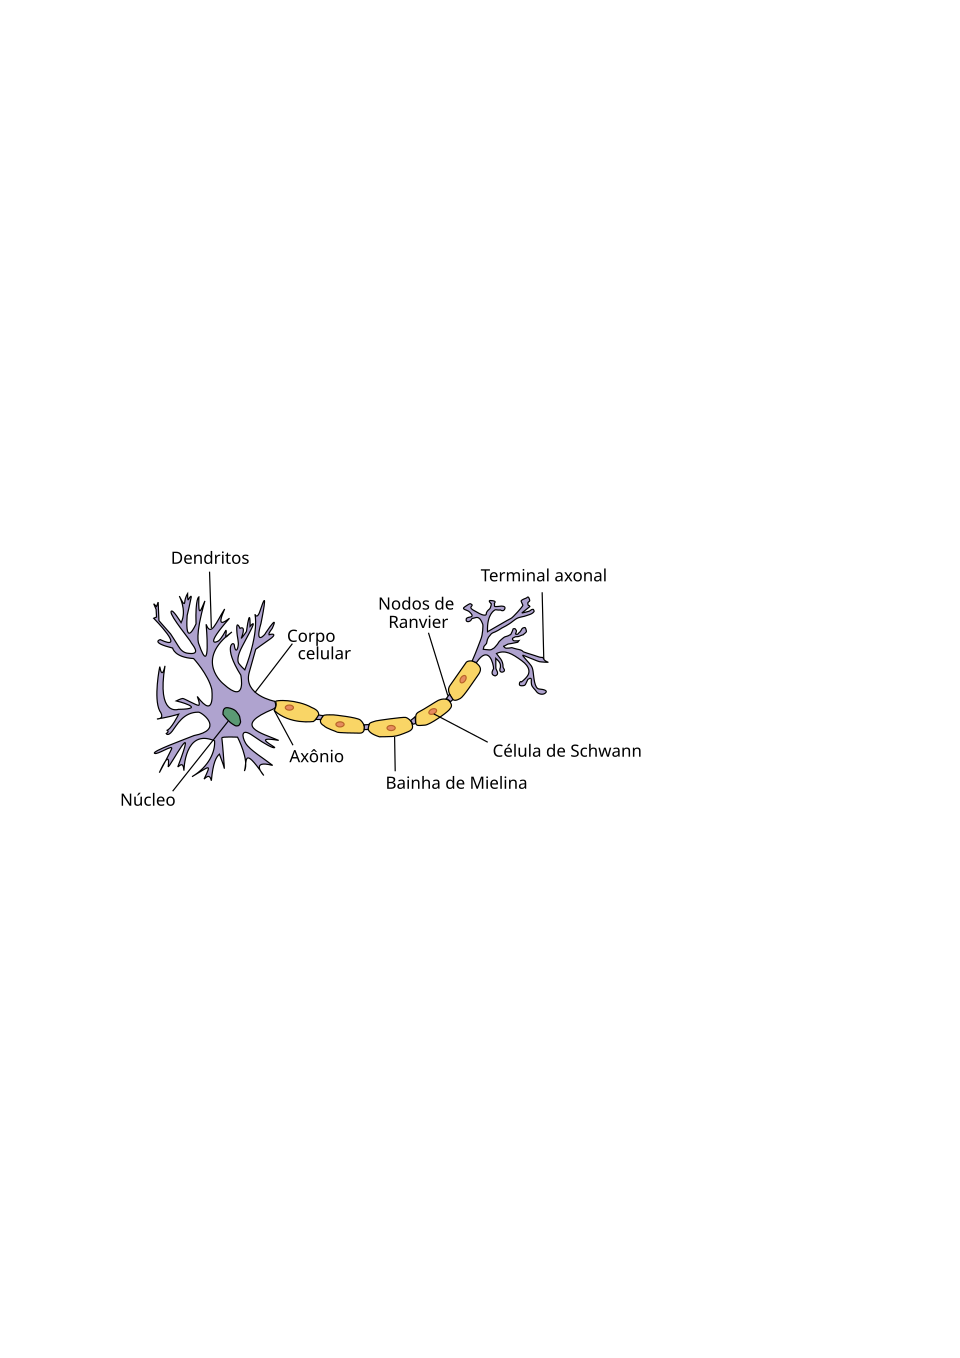
\includegraphics[width=\linewidth,trim=100 500 320 520,clip]{neuronio-biologico-wikimedia-ptbr.png}
        \caption{Neurônio biológico.}
        \label{fig:neuronio_biologico}
    \end{subfigure}
    \hfill
    \begin{subfigure}[t]{0.48\linewidth}
        \centering
        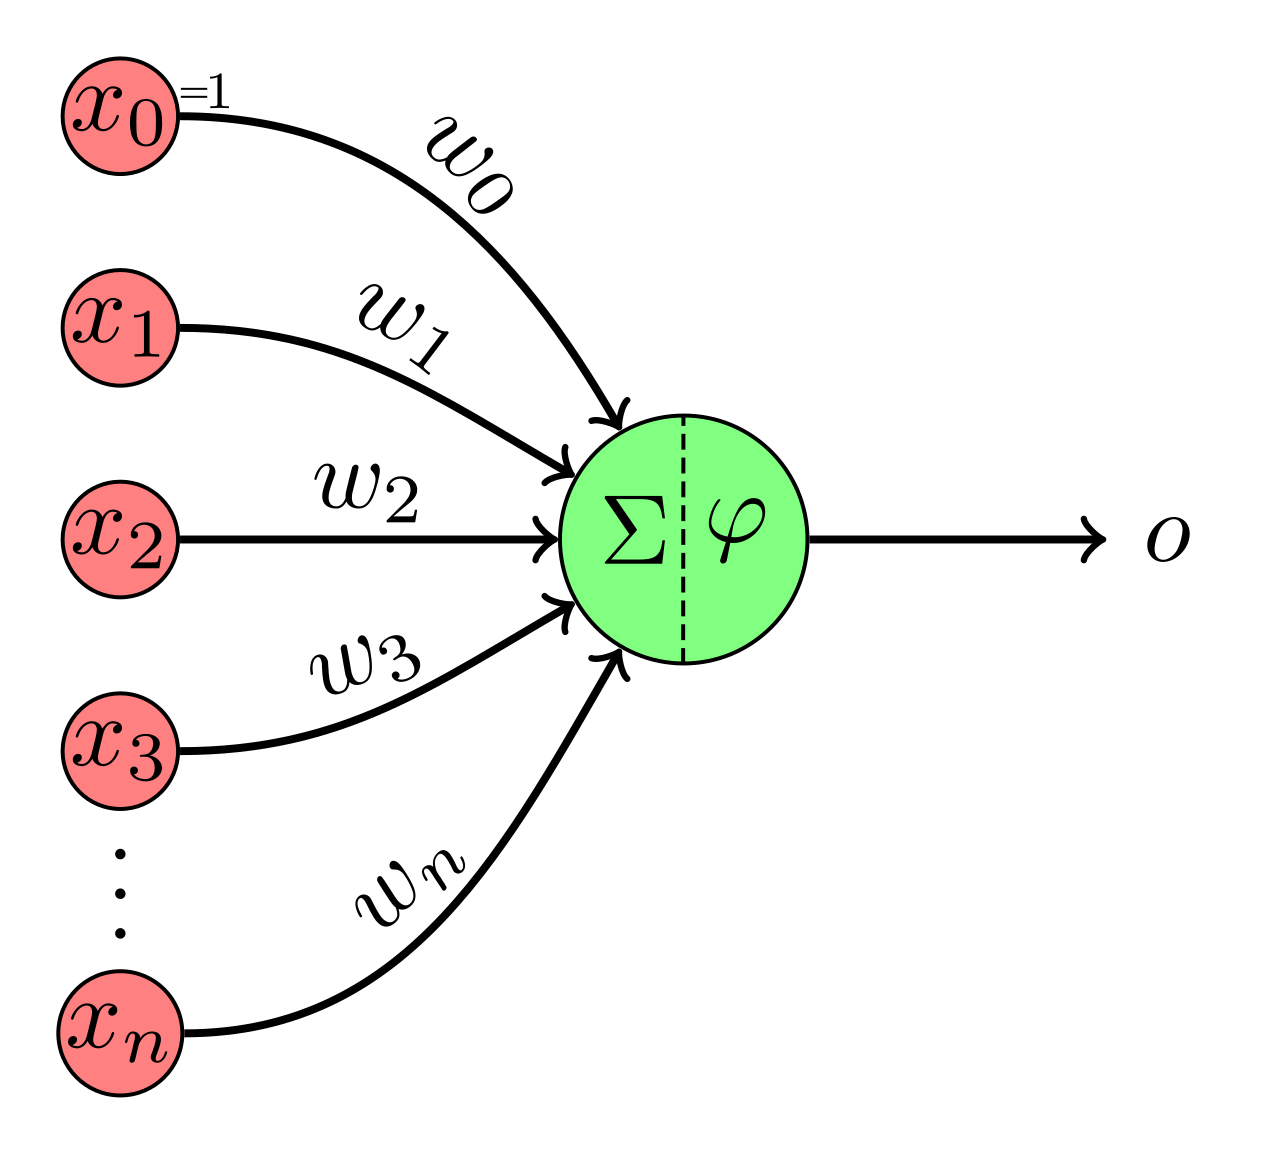
\includegraphics[width=0.86\linewidth]{neuronio-artificial-perceptron-wikimedia.png}
        \caption{Neurônio artificial.}
        \label{fig:neuronio_artificial_perceptron}
    \end{subfigure}
    \caption[Comparação visual entre neurônio biológico e neurônio artificial]{Comparação visual entre neurônio biológico e neurônio artificial. A imagem do neurônio biológico possui rótulos em português do Brasil e foi obtida de \citeonline{vasconcelos2008neuronPt}; a imagem do perceptron explicita entradas \(x_i\), pesos \(w_i\), soma ponderada, função de ativação \(\varphi\) e saída \(o\), conforme \citeonline{thoma2014perceptronUnit}.}
    \label{fig:neuronio_biologico_artificial}
\end{figure}

Formalmente, para um vetor de entrada $\mathbf{x}=(x_1,\ldots,x_d)$, um neurônio artificial calcula uma soma ponderada e aplica uma função de ativação:

\[
    a = \sum_{j=1}^{d} w_jx_j + b,
    \quad
    h = \phi(a).
\]

Nessa expressão, $w_j$ são pesos, $b$ é o viés, $a$ é a ativação antes da não linearidade e $\phi$ é uma função de ativação, como sigmoide, tangente hiperbólica ou unidade linear retificada (\textit{Rectified Linear Unit}, ReLU). Na Figura~\ref{fig:neuronio_artificial_perceptron}, o viés é representado por um peso \(w_0\) associado a uma entrada fixa \(x_0=1\), notação equivalente à adição explícita do termo \(b\). Os pesos e vieses são parâmetros aprendidos a partir dos dados. A função de ativação é importante porque introduz não linearidade; sem ela, uma composição de camadas lineares continuaria equivalente a uma única transformação linear.

Uma rede neural organiza vários neurônios em camadas. A saída de uma camada alimenta a camada seguinte, permitindo que o modelo componha transformações simples em representações mais complexas. De forma resumida, uma camada pode ser escrita como:

\[
    \mathbf{h}^{(\ell)}
    =
    \phi\left(
        W^{(\ell)}\mathbf{h}^{(\ell-1)}
        +
        \mathbf{b}^{(\ell)}
    \right),
\]

em que \(W^{(\ell)}\) e \(\mathbf{b}^{(\ell)}\) são os parâmetros da camada \(\ell\). O treinamento ajusta esses parâmetros para minimizar uma função de perda nos exemplos observados. Em tarefas de regressão, essa perda mede a distância entre os valores previstos e observados.

Aprendizado profundo, ou \textit{deep learning}, refere-se ao treinamento de redes neurais com múltiplas camadas e representações sucessivas dos dados \cite{goodfellow2016deep,lecun2015deep}. Em séries temporais, essa ideia é útil porque o modelo pode aprender relações não lineares entre medições recentes, variáveis exógenas, padrões cíclicos e o horizonte previsto. As arquiteturas recorrentes e codificador-decodificador discutidas nas seções seguintes são casos específicos de redes profundas voltadas a sequências: elas compartilham parâmetros ao longo do tempo, mantêm estados internos e produzem previsões para um ou mais horizontes futuros.

\section{Redes Neurais Recorrentes e Long Short-Term Memory (LSTM)}
\label{sec:rnn_lstm}

Redes neurais recorrentes (Recurrent Neural Networks, RNNs) são projetadas para dados sequenciais, pois atualizam um estado interno conforme processam cada instante da sequência. Em RNNs simples, o treinamento pode sofrer com desaparecimento ou explosão de gradientes, dificultando o aprendizado de dependências mais longas. A arquitetura Long Short-Term Memory (LSTM) introduz uma célula de memória e portões de entrada, esquecimento e saída para controlar o fluxo de informação \cite{hochreiter1997long}.

Uma célula LSTM pode ser descrita pelas seguintes equações, para entrada $\mathbf{x}_t$, estado oculto anterior $\mathbf{h}_{t-1}$ e memória anterior $\mathbf{c}_{t-1}$:

\[
\begin{aligned}
    \mathbf{i}_t &= \sigma(W_i\mathbf{x}_t + U_i\mathbf{h}_{t-1} + \mathbf{b}_i),\\
    \mathbf{f}_t &= \sigma(W_f\mathbf{x}_t + U_f\mathbf{h}_{t-1} + \mathbf{b}_f),\\
    \mathbf{o}_t &= \sigma(W_o\mathbf{x}_t + U_o\mathbf{h}_{t-1} + \mathbf{b}_o),\\
    \tilde{\mathbf{c}}_t &= \tanh(W_c\mathbf{x}_t + U_c\mathbf{h}_{t-1} + \mathbf{b}_c),\\
    \mathbf{c}_t &= \mathbf{f}_t \odot \mathbf{c}_{t-1} + \mathbf{i}_t \odot \tilde{\mathbf{c}}_t,\\
    \mathbf{h}_t &= \mathbf{o}_t \odot \tanh(\mathbf{c}_t).
\end{aligned}
\]

O portão de esquecimento $\mathbf{f}_t$ controla quanto da memória anterior é preservado; o portão de entrada $\mathbf{i}_t$ controla quanto da nova informação candidata é incorporado; e o portão de saída $\mathbf{o}_t$ controla a parte da memória exposta no estado oculto. A Figura~\ref{fig:lstm_propria} resume essa estrutura.

\begin{figure}[htbp]
    \centering
    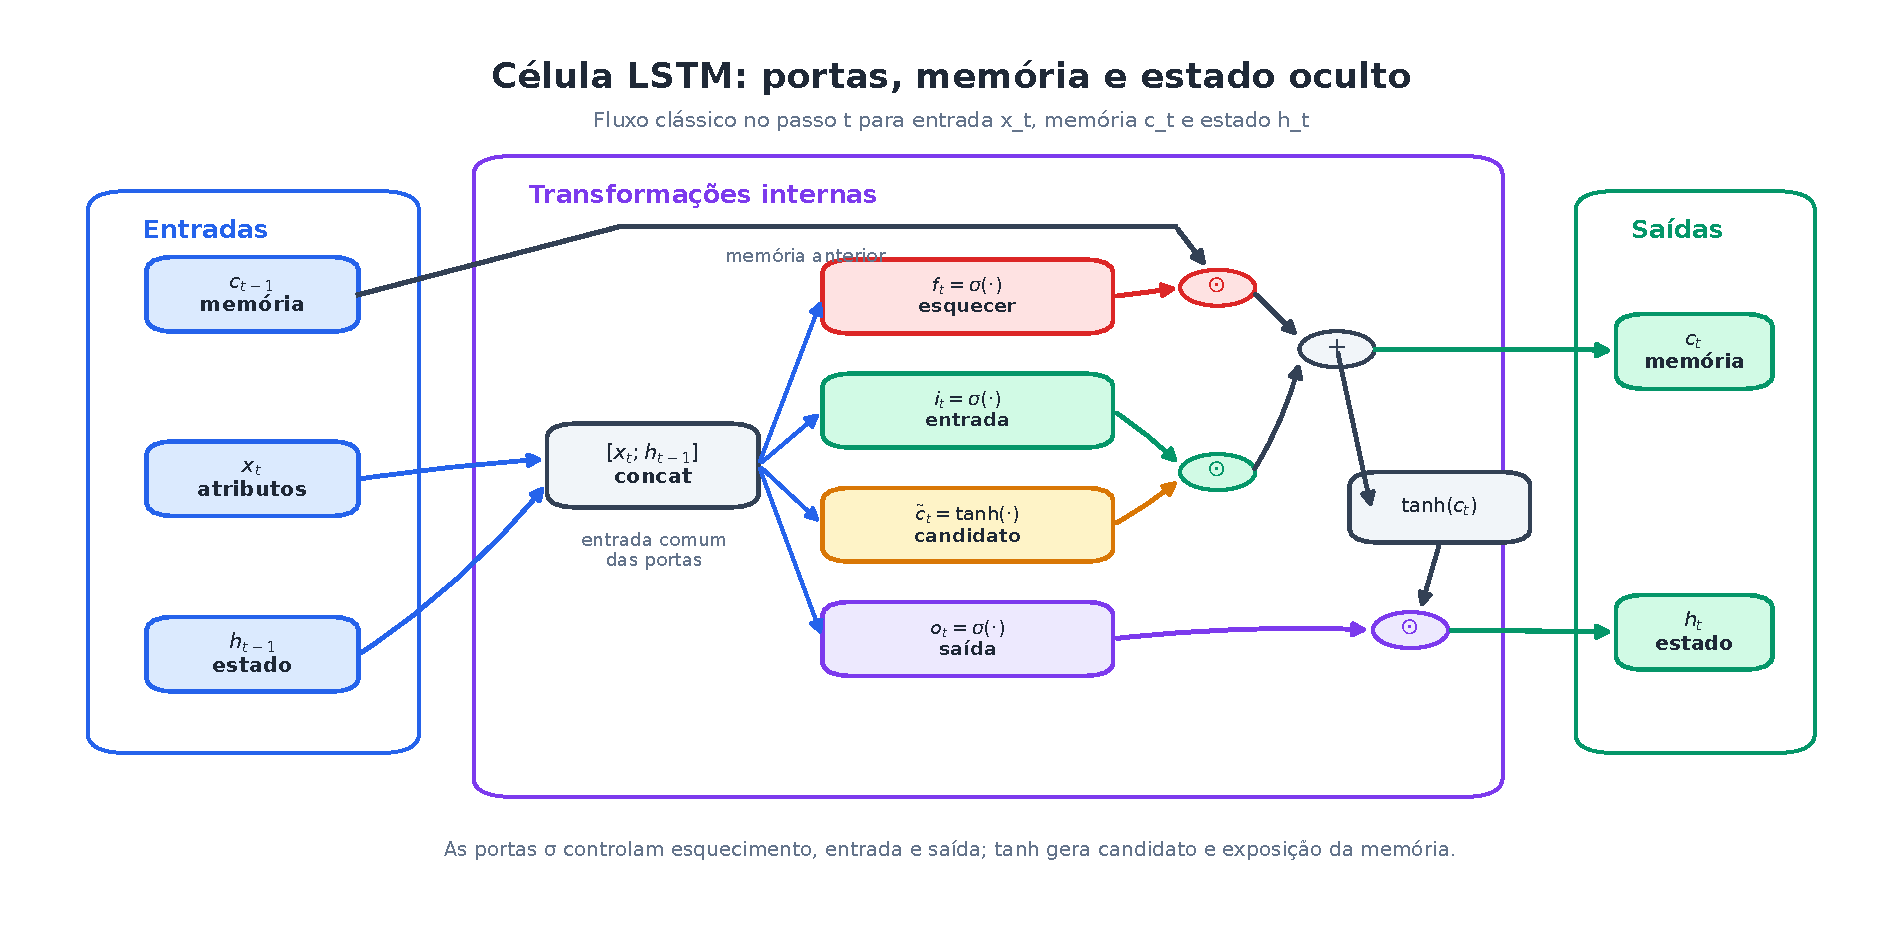
\includegraphics[width=0.95\textwidth]{diagrama_lstm_proprio.pdf}
    \caption{Diagrama conceitual de uma célula LSTM. Elaboração própria com base em \citeonline{hochreiter1997long}.}
    \label{fig:lstm_propria}
\end{figure}

Em previsão multi-horizonte, a LSTM pode ser usada em estratégias recursivas ou diretas. Na estratégia recursiva, o modelo aprende a avançar ao longo do horizonte com realimentação. Na estratégia direta, o estado final da janela de entrada é projetado para todo o horizonte futuro. A comparação entre essas estratégias permite separar o efeito da arquitetura recorrente do efeito da forma de gerar o horizonte.

\section{Sequence-to-Sequence (Seq2Seq) e Atenção}
\label{sec:encoder_decoder_attention}

Modelos \textit{Sequence-to-Sequence} (Seq2Seq) foram propostos para mapear uma sequência de entrada em uma sequência de saída. \citeonline{sutskever2014sequence} descrevem a proposta como uma abordagem ``\textit{end-to-end}'' para aprendizado de sequências, em que um codificador transforma a entrada em representação latente e um decodificador gera a sequência de saída. Em séries temporais, essa estrutura é útil porque o decodificador pode produzir um horizonte completo e receber variáveis conhecidas para cada horizonte futuro.

Sejam $\mathbf{h}_j$ os estados do codificador para os \(L\) instantes da janela de entrada. Uma formulação simplificada do codificador é:

\[
    \mathbf{h}_j = Enc_{\theta}(\mathbf{x}_{t-L+j}, \mathbf{h}_{j-1}), \quad j=1,\ldots,L.
\]

Sem atenção, o decodificador depende principalmente de um vetor de contexto, frequentemente associado ao último estado do codificador. A atenção reduz esse gargalo. O próprio trabalho de \citeonline{bahdanau2014neural} caracteriza o ``\textit{fixed-length vector}'' como uma limitação em tarefas sequência-para-sequência. Com atenção aditiva, para cada horizonte futuro \(k\), calculam-se escores, pesos normalizados e um contexto:

\[
\begin{aligned}
    e_{k,j} &= \mathbf{v}_a^{\top}\tanh(W_s\mathbf{s}_{k-1} + W_h\mathbf{h}_{j} + \mathbf{b}_a),\\
    \alpha_{k,j} &= \frac{\exp(e_{k,j})}{\sum_{\ell=1}^{L}\exp(e_{k,\ell})},\\
    \mathbf{c}_k &= \sum_{j=1}^{L}\alpha_{k,j}\mathbf{h}_j.
\end{aligned}
\]

O decodificador atualiza seu estado e produz a previsão:

\[
\begin{aligned}
    \mathbf{s}_k &= Dec_{\theta}(\mathbf{s}_{k-1}, \tilde{y}_{t+k-1}, \mathbf{z}_{t+k}, \mathbf{c}_k),\\
    \hat{y}_{t+k} &= g_{\theta}(\mathbf{s}_k, \mathbf{c}_k, \mathbf{z}_{t+k}).
\end{aligned}
\]

Nessas expressões, \(W_s\), \(W_h\), \(\mathbf{v}_a\) e \(\mathbf{b}_a\) são parâmetros aprendidos do mecanismo de atenção, enquanto \(\mathbf{s}_k\) representa o estado do decodificador no horizonte \(k\).

Nesse caso, $\tilde{y}_{t+k-1}$ representa o valor real anterior durante \textit{teacher forcing} ou a previsão anterior durante inferência. Variações de atenção global e local também foram propostas, incluindo mecanismos do tipo Luong \cite{luong2015effective}. Para séries temporais multivariadas, arquiteturas como Dual-stage Attention-based Recurrent Neural Network (DA-RNN) combinam atenção sobre variáveis de entrada e atenção temporal \cite{qin2017darnn}.

A utilidade de Seq2Seq em previsão não se apoia na ideia de que essa família seja sempre superior. A justificativa é mais específica: tarefas multi-horizonte podem se beneficiar de um decodificador condicionado por atributos futuros conhecidos e trabalhos de previsão adotam estruturas recorrentes sequência-para-sequência para prever uma sequência de horizontes futuros. Por exemplo, \citeonline{wen2017mqrnn} exploram a natureza temporal de ``\textit{Sequence-to-Sequence Neural Networks}'' em previsão multi-horizonte, enquanto DeepAR e Temporal Fusion Transformer exemplificam linhas modernas de previsão profunda com decodificadores autoregressivos, covariáveis e previsão multi-horizonte \cite{salinas2020deepar,lim2021tft}. A Figura~\ref{fig:seq2seq_attention_propria} sintetiza uma formulação conceitual de Seq2Seq com atenção.

\begin{figure}[htbp]
    \centering
    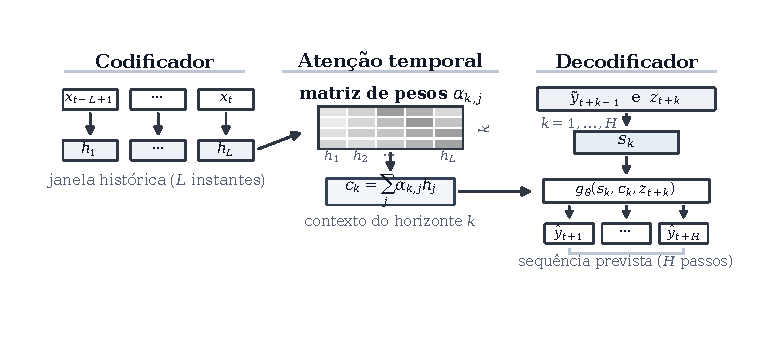
\includegraphics[width=0.95\textwidth]{diagrama_seq2seq_attention_proprio.pdf}
    \caption[Seq2Seq com atenção]{Diagrama conceitual de Seq2Seq com atenção para previsão multi-horizonte. Elaboração própria com base em \citeonline{sutskever2014sequence}, \citeonline{bahdanau2014neural}, \citeonline{luong2015effective} e \citeonline{qin2017darnn}.}
    \label{fig:seq2seq_attention_propria}
\end{figure}

Pesos de atenção não devem ser interpretados automaticamente como explicação causal \cite{jain2019attention} nem como garantia de superioridade. Eles podem ser pouco informativos quando ficam quase uniformes ou quando não produzem ganho mensurável em avaliação fora da amostra.

\section{\textit{Teacher Forcing} e \textit{Scheduled Sampling}}

Em modelos com decodificador autoregressivo, o treinamento pode usar \textit{teacher forcing}: em vez de alimentar a previsão anterior do próprio modelo, usa-se o valor observado anterior como entrada do próximo instante. Isso acelera o treinamento, mas cria diferença entre treino e inferência, já que o valor real futuro não está disponível no momento da previsão. \citeonline{bengio2015scheduled} descrevem esse problema como discrepância entre treinamento e inferência, pois o item anterior verdadeiro está disponível no treino, mas é substituído por uma saída gerada pelo próprio modelo na inferência.

Seja \(p_{TF}\) a probabilidade de usar o valor real anterior no decodificador. Em cada horizonte futuro \(k\), pode-se sortear \(b_{i,k}\sim\text{Bernoulli}(p_{TF})\) e definir a entrada autoregressiva como:

\[
    \tilde{y}_{t+k-1}
    =
    b_{i,k}y_{t+k-1}
    +
    (1-b_{i,k})\hat{y}_{t+k-1}.
\]

Quando \(p_{TF}=1\), o modelo opera em \textit{teacher forcing} puro; quando \(p_{TF}=0\), ele treina de modo equivalente à inferência autoregressiva, sempre realimentando suas próprias previsões. O \textit{scheduled sampling} clássico propõe variar \(p_{TF}\) ao longo do treinamento, geralmente reduzindo essa probabilidade para deslocar gradualmente o decodificador de um regime totalmente guiado para um regime menos guiado e mais próximo da inferência \cite{bengio2015scheduled}.

Para previsão de séries temporais contínuas, entretanto, há uma motivação adicional para testar a direção oposta. \citeonline{teutsch2022flipped} argumentam que o \textit{scheduled sampling} clássico, herdado de tarefas de processamento de linguagem natural (Natural Language Processing, NLP), pode não ser a estratégia mais adequada para previsão e propõem currículos de \textit{Increasing Teacher Forcing}, denominados \textit{Flipped Classroom}. Nessa família, o treinamento começa mais próximo de \textit{free running}, com baixo \(p_{TF}\), e aumenta gradualmente a presença de \textit{teacher forcing}. Em experimentos com sistemas dinâmicos, os autores relataram ganhos de aproximadamente 15\% a 80\% na raiz do erro quadrático médio normalizado (Normalized Root Mean Squared Error, NRMSE) em previsão multi-horizonte em relação à melhor configuração de referência de \textit{teacher forcing} ou \textit{free running}, embora limitem a conclusão ao escopo experimental avaliado.

\clearpage

\begin{figure}[htbp]
    \centering
    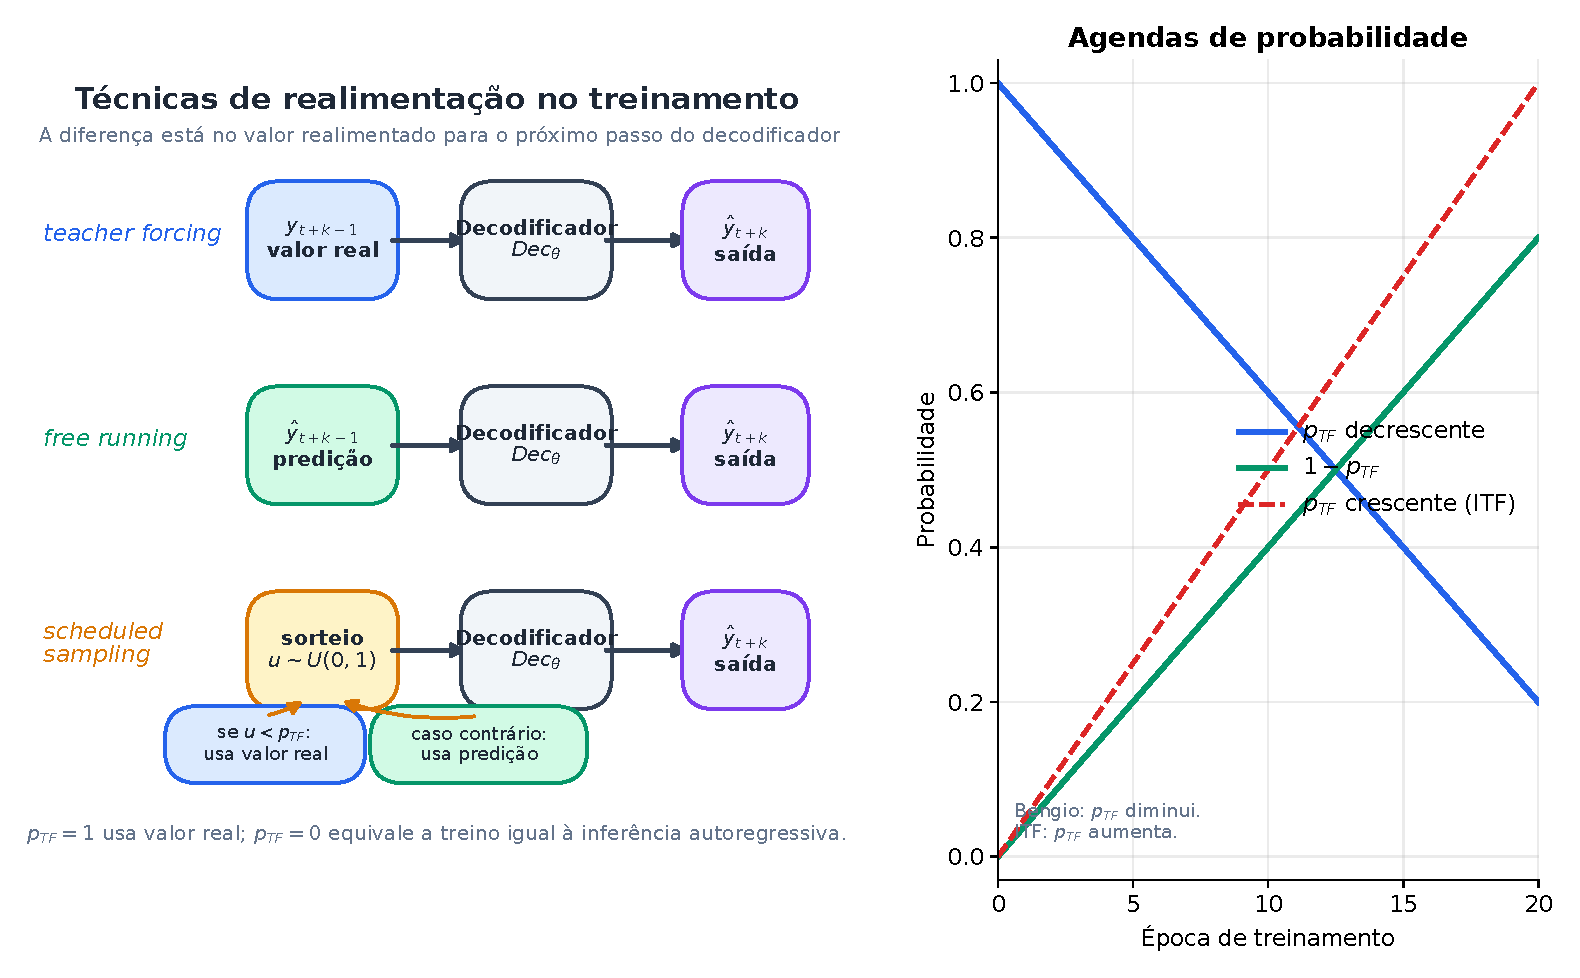
\includegraphics[width=\linewidth]{teacher_forcing_scheduled_sampling.pdf}
    \caption[\textit{Teacher forcing}, \textit{scheduled sampling} e agenda crescente]{Comparação entre \textit{teacher forcing}, inferência autoregressiva, \textit{scheduled sampling} clássico e agenda crescente de \textit{teacher forcing}. Elaboração própria com base em \citeonline{bengio2015scheduled} e \citeonline{teutsch2022flipped}.}
    \label{fig:teacher_forcing_scheduled_sampling}
\end{figure}

A notação da Figura \ref{fig:teacher_forcing_scheduled_sampling} é importante: \(p_{TF}\) representa a probabilidade de usar o valor real anterior. Assim, uma agenda decrescente de \(p_{TF}\) aumenta o uso das próprias previsões do modelo e corresponde à intuição original do \textit{scheduled sampling}; já uma agenda crescente de \(p_{TF}\) aumenta a dependência de \textit{teacher forcing} e se aproxima da hipótese de \textit{Increasing Teacher Forcing}. Essa distinção evita confundir a direção da agenda de treinamento com a interpretação do regime autoregressivo.

\clearpage

\section{Impulsionamento por Gradiente e Extreme Gradient Boosting (XGBoost)}

Modelos de árvores com impulsionamento (\textit{boosting}) constroem um preditor aditivo por meio de várias árvores fracas, ajustadas sequencialmente para corrigir erros residuais. O \textit{Extreme Gradient Boosting} (XGBoost) é uma implementação eficiente de impulsionamento por gradiente (\textit{gradient boosting}) com regularização, paralelização e recursos práticos para matrizes de atributos \cite{chen2016xgboost}. Neste trabalho, essa matriz representa janelas temporais transformadas em atributos numéricos para uma tarefa supervisionada. Por lidar bem com atributos defasados e variáveis derivadas, o XGBoost é frequentemente usado como modelo de referência para previsão de séries temporais transformadas nesse formato.

No impulsionamento aditivo, a predição após $K$ árvores pode ser escrita como:

\[
    \hat{y}_i^{(K)} = \sum_{k=1}^{K} f_k(\mathbf{u}_i), \quad f_k \in \mathcal{F},
\]

em que $\mathbf{u}_i$ é o vetor de atributos derivado da janela temporal. O objetivo regularizado do XGBoost pode ser representado por:

\[
    \mathcal{L}^{(K)}
    =
    \sum_i \ell(y_i, \hat{y}_i^{(K)})
    +
    \sum_{k=1}^{K}\Omega(f_k),
    \quad
    \Omega(f_k)=\gamma T_k + \frac{1}{2}\lambda\lVert\mathbf{w}_k\rVert_2^2.
\]

Nessa expressão, $T_k$ é o número de folhas da árvore e $\mathbf{w}_k$ são os pesos das folhas. A regularização penaliza árvores excessivamente complexas e ajuda a controlar sobreajuste. Em problemas multi-horizonte, o XGBoost pode ser combinado com estratégias de saída múltipla para prever todo o horizonte futuro de uma vez; a Figura~\ref{fig:xgboost_multioutput_propria} ilustra essa conversão por janelas.

\begin{figure}[htbp]
    \centering
    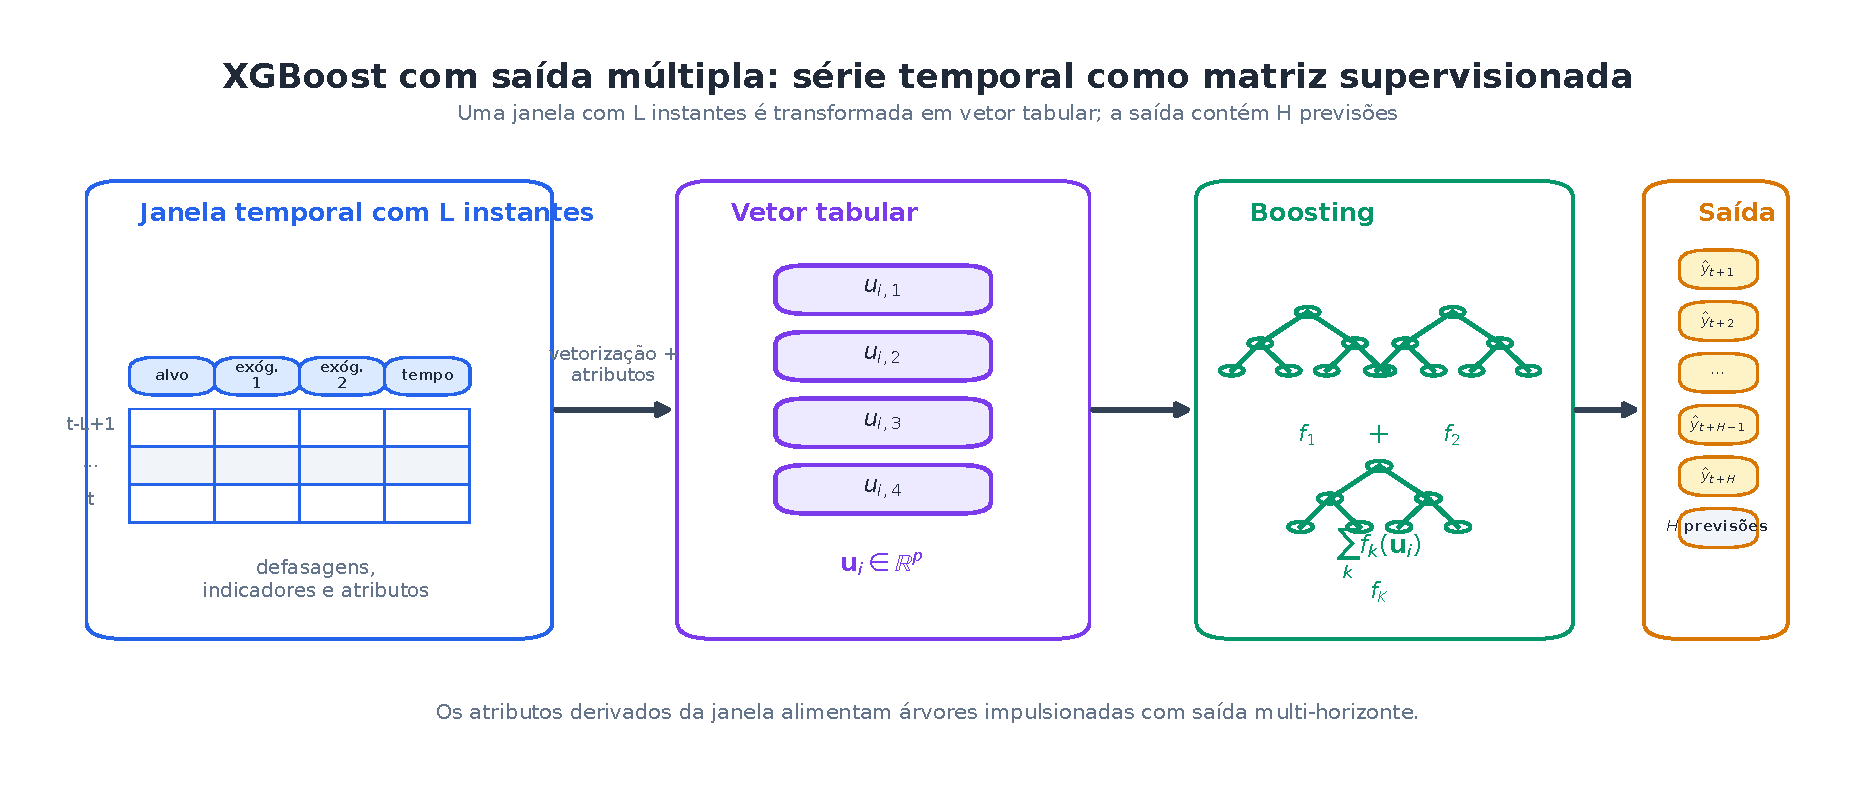
\includegraphics[width=0.90\textwidth]{diagrama_xgboost_multioutput_proprio.pdf}
    \caption{Conversão de uma janela temporal em matriz de atributos para XGBoost com saída múltipla. Elaboração própria com base em \citeonline{chen2016xgboost}.}
    \label{fig:xgboost_multioutput_propria}
\end{figure}

Em aplicações com dados faltantes, a conversão por janelas precisa manter consistência entre as entradas, o horizonte previsto e os critérios de inclusão de alvos observados. Essa decisão afeta a comparabilidade entre modelos baseados em árvores e modelos neurais quando há máscaras ou perdas definidas ponto a ponto.

\section{Treinamento, Função de Perda e Otimização de Hiperparâmetros}
\label{sec:otimizacao_hpo}

Parâmetros são aprendidos pelo modelo durante o treinamento; hiperparâmetros, como taxa de aprendizado, número de camadas, tamanho do estado oculto e \textit{dropout}, são definidos antes ou buscados por procedimento externo. Essa busca é chamada de otimização de hiperparâmetros, indicada neste trabalho pela sigla HPO, do inglês \textit{Hyperparameter Optimization}. Redes neurais são frequentemente treinadas com otimizadores baseados em gradiente, como Adam e AdamW \cite{kingma2014adam,loshchilov2019decoupled}, e podem usar monitoramento em validação para seleção de ponto de controle.

A taxa de aprendizado controla o tamanho do passo aplicado aos parâmetros a cada atualização por gradiente. Ela pode ser mantida constante ou seguir uma agenda ao longo das épocas. Uma estratégia comum combina aquecimento linear (\textit{linear warm-up}) e decaimento cosseno: o aquecimento linear aparece em protocolos de treinamento com lotes grandes \cite{goyal2017accurate}, enquanto agendas cossenoidais são discutidas no contexto de reinícios quentes \cite{loshchilov2017sgdr}. Com \(E_w\) épocas de aquecimento, \(E\) épocas máximas, taxa máxima \(\eta_{\max}\) e taxa mínima \(\eta_{\min}\), a forma idealizada é:

\[
    \eta_t =
    \begin{cases}
        \eta_{\max}\left(10^{-5} + (1-10^{-5})\frac{t}{E_w}\right), & 0 \leq t \leq E_w,\\
        \eta_{\min} + \frac{1}{2}(\eta_{\max}-\eta_{\min})\left[1+\cos\left(\pi\frac{t-E_w}{E-E_w}\right)\right], & E_w < t \leq E.
    \end{cases}
\]

Assim, as primeiras épocas usam passos pequenos e aumentam gradualmente a taxa até \(\eta_{\max}\). Depois do aquecimento, a taxa decai suavemente até \(\eta_{\min}\). Essa variação ocorre por época durante o treinamento. A etapa de validação, por sua vez, não aplica retropropagação nem atualiza os pesos; ela avalia o modelo no fim das épocas e fornece métricas para parada antecipada, escolha de ponto de controle e poda de tentativas na HPO. Portanto, a validação influencia a seleção e a interrupção de treinamentos, mas não ajusta diretamente a taxa de aprendizado como ocorreria em uma agenda dependente da métrica de validação.

Também são usadas funções de perda robustas ou ponderadas. A perda de Huber combina comportamento quadrático para erros pequenos e linear para erros grandes, reduzindo a sensibilidade a outliers em comparação com o erro quadrático puro \cite{huber1964robust}. Para erro $e=y-\hat{y}$, ela é definida por:

\[
    \ell_{\delta}(e)=
    \begin{cases}
        \frac{1}{2}e^2, & \text{se } |e| \leq \delta,\\
        \delta\left(|e|-\frac{1}{2}\delta\right), & \text{caso contrário}.
    \end{cases}
\]

Quando um conjunto de dados contém valores imputados no alvo, a função de perda e as métricas de avaliação podem usar uma máscara \(m_{i,k}\) que vale 1 quando o alvo do exemplo \(i\) e horizonte \(k\) foi observado e 0 quando foi imputado. Essa escolha segue a distinção entre valor observado e valor ausente ou estimado, além do uso de máscaras de observação em métodos de imputação temporal \cite{rubin1976inference,cao2018brits,du2023saits}:

\[
    \mathcal{J}(\theta)
    =
    \frac{\sum_{i,k}m_{i,k}\ell(y_{i,k}, \hat{y}_{i,k})}
    {\sum_{i,k}m_{i,k}}.
\]

Uma perda absoluta ponderada altera explicitamente o objetivo para atribuir maior peso a determinados regimes de concentração ou tipos de erro:

\[
    \mathcal{J}_{w}(\theta)
    =
    \frac{\sum_{i,k}m_{i,k}w_{i,k}|y_{i,k}-\hat{y}_{i,k}|}
    {\sum_{i,k}m_{i,k}w_{i,k}}.
\]

Essa formulação não é regularização L1 dos parâmetros; é uma perda absoluta ponderada no espaço das previsões. Por isso, eventuais mudanças de comportamento em picos ou cauda devem ser interpretadas como consequência de uma mudança de objetivo, e não como simples ganho arquitetural.

O Optuna é uma ferramenta para HPO com definição dinâmica de espaços de busca, estratégias de amostragem e poda de tentativas pouco promissoras \cite{akiba2019optuna}. Formalmente, seja $\lambda \in \Lambda$ um vetor de hiperparâmetros no espaço de busca $\Lambda$ e seja $A(D_{treino};\lambda)$ o algoritmo de treinamento com essa configuração. Em uma validação simples, o objetivo da HPO seria selecionar a configuração com menor erro de validação:

\[
    \lambda^{*}
    =
    \arg\min_{\lambda \in \Lambda}
    \mathcal{L}_{val}\left(A(D_{treino};\lambda), D_{val}\right).
\]

Em séries temporais, esse termo de validação pode ser substituído pela média das partições temporais, isto é, pela métrica \(\mathcal{L}_{CV}\) da validação \textit{walk-forward}. Assim, a escolha de \(\lambda^{*}\) pode usar várias origens temporais dentro do desenvolvimento, sem consultar uma avaliação final reservada.

No Optuna, cada tentativa, ou \textit{trial}, escolhe um ponto $\lambda$ do espaço de busca, treina o modelo com esse ponto e retorna uma métrica objetivo. O conjunto de tentativas forma um estudo (\textit{study}). A cada tentativa, o amostrador usa o histórico de configurações já avaliadas para propor novos hiperparâmetros. No caso padrão de otimização mono-objetivo, o Optuna usa o \texttt{TPESampler} como amostrador padrão \cite{optunaDocsEfficient2026}. O TPE, ou \textit{Tree-structured Parzen Estimator}, separa os valores de hiperparâmetros associados aos melhores resultados dos demais, ajusta modelos probabilísticos para esses dois grupos e tende a escolher novos valores que maximizem a razão entre regiões promissoras e não promissoras \cite{optunaDocsTPE2026}.

A poda, ou \textit{pruning}, é uma forma de parada antecipada no nível da HPO. Em vez de treinar todas as configurações até o orçamento máximo, o treinamento reporta valores intermediários de validação; o mecanismo de poda decide se uma tentativa deve continuar ou ser interrompida. O \texttt{HyperbandPruner} combina múltiplas instâncias de \textit{Successive Halving}, chamadas de chaves (\textit{brackets}), para distribuir orçamento entre muitas configurações baratas e poucas configurações que recebem mais épocas \cite{li2018hyperband,optunaDocsHyperband2026}. A própria documentação do Optuna apresenta o \texttt{HyperbandPruner} como uma combinação recomendada com \texttt{TPESampler} em resultados de referência para tarefas mono-objetivo \cite{optunaDocsEfficient2026}. Mesmo assim, HPO com orçamento limitado não deve ser interpretada como garantia de ótimo global.

\section{Métricas de Avaliação}
\label{sec:metricas_avaliacao}

A avaliação de modelos de regressão multi-horizonte deve combinar métricas globais e métricas por horizonte. Métricas como erro médio absoluto (\textit{Mean Absolute Error}, MAE), raiz do erro quadrático médio (\textit{Root Mean Squared Error}, RMSE) e erro percentual médio absoluto (\textit{Mean Absolute Percentage Error}, MAPE) são amplamente usadas para avaliar desempenho preditivo \cite{hyndman2021forecasting}. O MAE mede a magnitude média dos erros e é menos sensível a valores extremos que o erro quadrático:

\[
    \text{MAE}(y, \hat{y}) =
    \frac{1}{N}\sum_{i=1}^{N}|y_i - \hat{y}_i|.
\]

A raiz do erro quadrático médio (RMSE) penaliza erros grandes com mais intensidade:

\[
    \text{RMSE}(y, \hat{y}) =
    \sqrt{\frac{1}{N}\sum_{i=1}^{N}(y_i - \hat{y}_i)^2}.
\]

O erro percentual médio absoluto (MAPE) expressa o erro relativo em percentual, com cuidado adicional para valores próximos de zero:

\[
    \text{MAPE}(y, \hat{y}) =
    \frac{100}{N}\sum_{i=1}^{N}\left|\frac{y_i-\hat{y}_i}{|y_i|+\epsilon}\right|.
\]

O coeficiente de determinação ($R^2$) compara o erro do modelo com a variância do alvo:

\[
    R^2(y, \hat{y}) =
    1 - \frac{\sum_{i=1}^{N}(y_i - \hat{y}_i)^2}{\sum_{i=1}^{N}(y_i - \bar{y})^2}.
\]

Quando há valores imputados no alvo, as métricas devem ser calculadas apenas sobre os pontos originalmente observados, usando a mesma lógica da máscara \(m_i\). Para o MAE observado, por exemplo:

\[
    \text{MAE}_{obs}(y, \hat{y}) =
    \frac{\sum_{i=1}^{N}m_i|y_i-\hat{y}_i|}
    {\sum_{i=1}^{N}m_i}.
\]

O mesmo princípio se aplica a RMSE, MAPE e métricas por horizonte. No caso do \(R^2\), a média \(\bar{y}\) e as somas do numerador e do denominador devem ser calculadas no mesmo subconjunto observado. Isso evita tratar valores imputados como verdade de referência e mantém a avaliação vinculada às medições efetivamente observadas \cite{rubin1976inference,cao2018brits,du2023saits}.

Além dessas métricas globais, análises por horizonte, viés médio, percentis altos previstos e erro em eventos de maior concentração podem complementar a avaliação. Essa combinação é necessária porque um modelo pode vencer em erro médio e ainda produzir curvas excessivamente suavizadas, subestimando picos relevantes para a interpretação ambiental.

\clearpage

\section{Resumo do Capítulo}

Este capítulo definiu a base teórica do estudo: PM2,5 como série temporal ambiental, componentes temporais, autocorrelação, previsão multi-horizonte, tratamento de dados faltantes sem vazamento, janelas supervisionadas, variáveis exógenas disponíveis no momento da previsão, redes neurais artificiais, aprendizado profundo, LSTM, Seq2Seq com atenção, \textit{scheduled sampling}, XGBoost, HPO e métricas. A formulação matemática deixa explícita a distinção entre arquiteturas recorrentes, codificador-decodificador e modelos baseados em árvores, preparando a metodologia comparativa dos capítulos seguintes.

% cap_relacionados.tex
\chapter{Trabalhos Relacionados}
\label{chap:trabalhos_relacionados}

A previsão da concentração de PM2.5 utilizando métodos de aprendizado de máquina e aprendizado profundo é uma área de pesquisa ativa. Diversos estudos têm explorado diferentes arquiteturas e abordagens para melhorar a acurácia das previsões.

O trabalho de \citeonline{yang2023attention} utilizou um modelo LSTM com mecanismo de atenção, demonstrando que esta combinação melhora a precisão da previsão em comparação com modelos como ARIMA, AutoEncoder e LSTM padrão. De forma similar, \citeonline{zhao2021pm2} combinaram a Decomposição por Modos Empíricos (EMD) com LSTM, alcançando uma redução significativa no erro absoluto médio (MAE). Esses estudos corroboram a hipótese de que a personalização de arquiteturas LSTM baseadas nas características dos dados pode levar a ganhos de desempenho.

Métodos tradicionais de aprendizado de máquina, como Máquinas de Vetores de Suporte (SVM) e Florestas Aleatórias, também foram aplicados com sucesso. \citeonline{song2018arima} otimizaram um modelo de regressão de vetores de suporte com um algoritmo de lobo cinzento, enquanto \citeonline{guo2019pm2} integraram parâmetros meteorológicos de GNSS em um modelo de floresta aleatória, ambos mostrando a importância da engenharia de atributos e da otimização de modelos.

Estudos mais recentes exploram arquiteturas de deep learning ainda mais complexas. \citeonline{zhang2021deep} propuseram um modelo Bi-Direcional com LSTM Aninhado (BiNLSTM), que se mostrou superior ao LSTM padrão ao capturar informações de longo prazo de forma mais eficaz. \citeonline{yuan2020using} aplicaram uma rede Encoder-Decoder com atenção, similar à abordagem deste trabalho, para detecção de perturbações em séries temporais de sensoriamento remoto, destacando a versatilidade da arquitetura.

O presente estudo se diferencia e contribui para a literatura existente ao realizar uma \textbf{análise comparativa sistemática} de uma progressão de modelos, desde LSTMs simples até um Encoder-Decoder com atenção e \textit{Scheduled Sampling}. Além disso, adota uma abordagem de \textbf{previsão probabilística} para quantificar a incerteza e utiliza uma técnica de imputação de dados estado da arte (\textbf{SAITS}), fornecendo uma análise metodológica abrangente e rigorosa para o contexto específico das estações de monitoramento em Minas Gerais.
% cap_metodologia.tex
\chapter{Materiais e Métodos}
\label{chap:materiais_metodos}

Este capítulo descreve o protocolo experimental utilizado na comparação dos modelos. A metodologia foi definida para preservar a ordem temporal dos dados, evitar vazamento de informação futura e permitir comparação direta entre arquiteturas sob o mesmo contrato de entrada, saída e avaliação.

\section{Fonte de Dados e Escopo}

O estudo utiliza medições horárias da estação Sapo, localizada em Conceição do Mato Dentro, Minas Gerais. Neste trabalho, a sigla CMD é usada apenas como abreviação do município de Conceição do Mato Dentro quando necessário. Os dados fazem parte do monitoramento contínuo de qualidade do ar disponibilizado pela Fundação Estadual do Meio Ambiente de Minas Gerais (FEAM) \cite{feam2026dadosmonitoramento}. A variável-alvo é a concentração de material particulado fino (PM2,5), e o principal poluente auxiliar mantido no contrato final é o material particulado com diâmetro de até 10 micrômetros (PM10). O conjunto original também contém variáveis meteorológicas e gases, mas essas colunas foram removidas do contrato principal porque apresentavam alta esparsidade na estação Sapo e prejudicavam a coerência do conjunto de dados final.

O conjunto consolidado usado nos resultados principais contém 34.991 registros horários, de 2017-01-04 00:30:00 a 2020-12-31 22:30:00. Esse período corresponde ao recorte efetivamente disponível após preparação, criação das variáveis substitutas causais de PM10 e remoção das primeiras janelas necessárias para a formulação supervisionada.

\begin{table}[htb]
    \centering
    \caption{Resumo do contrato experimental principal.}
    \label{tab:contrato_experimental}
    \resizebox{\textwidth}{!}{%
    \begin{tabular}{ll}
        \toprule
        \textbf{Item} & \textbf{Definição} \\
        \midrule
        Estação & Sapo / CMD (Conceição do Mato Dentro, Minas Gerais) \\
        Poluente-alvo & PM2,5 horário \\
        Período do artefato & 2017-01-04 00:30:00 a 2020-12-31 22:30:00 \\
        Número de linhas & 34.991 \\
        Tarefa & 48 horas passadas para prever as próximas 24 horas \\
        Divisão externa & Cronológica por proporção 70/15/15 \\
        Seleção de hiperparâmetros & \textit{Walk-forward} temporal nos 85\% anteriores ao teste \\
        Imputação & Linear no contrato final, com máscaras de valores originalmente ausentes \\
        Variáveis principais & PM2,5, PM10, indicadores de ausência, tempo/Fourier e substitutos causais de PM10 \\
        Avaliação final & Teste externo, sem embaralhamento temporal \\
        \bottomrule
    \end{tabular}%
    }
\end{table}

\section{Análise Exploratória e Escolha da Estação}

A escolha da estação Sapo foi precedida por uma análise exploratória comparativa sobre 38 estações/usinas com PM2,5. Essa etapa combinou critérios de cobertura do alvo, continuidade temporal, presença de PM10 pareado, frequência de eventos altos e equilíbrio das partições cronológicas. O objetivo dessa triagem não foi escolher uma estação apenas por conveniência, mas selecionar um recorte com volume suficiente, variável auxiliar causalmente útil e incidência mínima de eventos de cauda para sustentar a comparação entre modelos.

Nesse diagnóstico, Sapo apareceu como uma das candidatas mais fortes: ficou em segundo lugar na classificação por PM2,5 puro e também em segundo lugar na classificação que inclui contexto de PM10. A estação Rio Doce/Estação Principal obteve pontuação ligeiramente maior, mas teve menor frequência de eventos PM2,5 \(\geq 35\) no diagnóstico preliminar (0,19\%, contra 1,16\% em Sapo) e não pertence ao mesmo foco CMD adotado neste trabalho. Assim, Sapo foi mantida como estação principal por combinar aderência ao escopo, cobertura de PM2,5 de 83,47\% no diagnóstico comparativo, cobertura pareada PM10 de 74,27\% e correlação absoluta PM10--PM2,5 de 0,58.

Essa escolha deve ser lida como um recorte metodológico do estudo, não como afirmação de que Sapo seja a estação mais previsível de toda a rede. O papel da triagem foi selecionar uma estação com dados suficientes, presença de PM10 auxiliar e eventos altos em quantidade mínima para análise de cauda. A generalização para outras estações permanece uma limitação e uma possibilidade de continuidade.

\begin{figure}[htb]
    \centering
    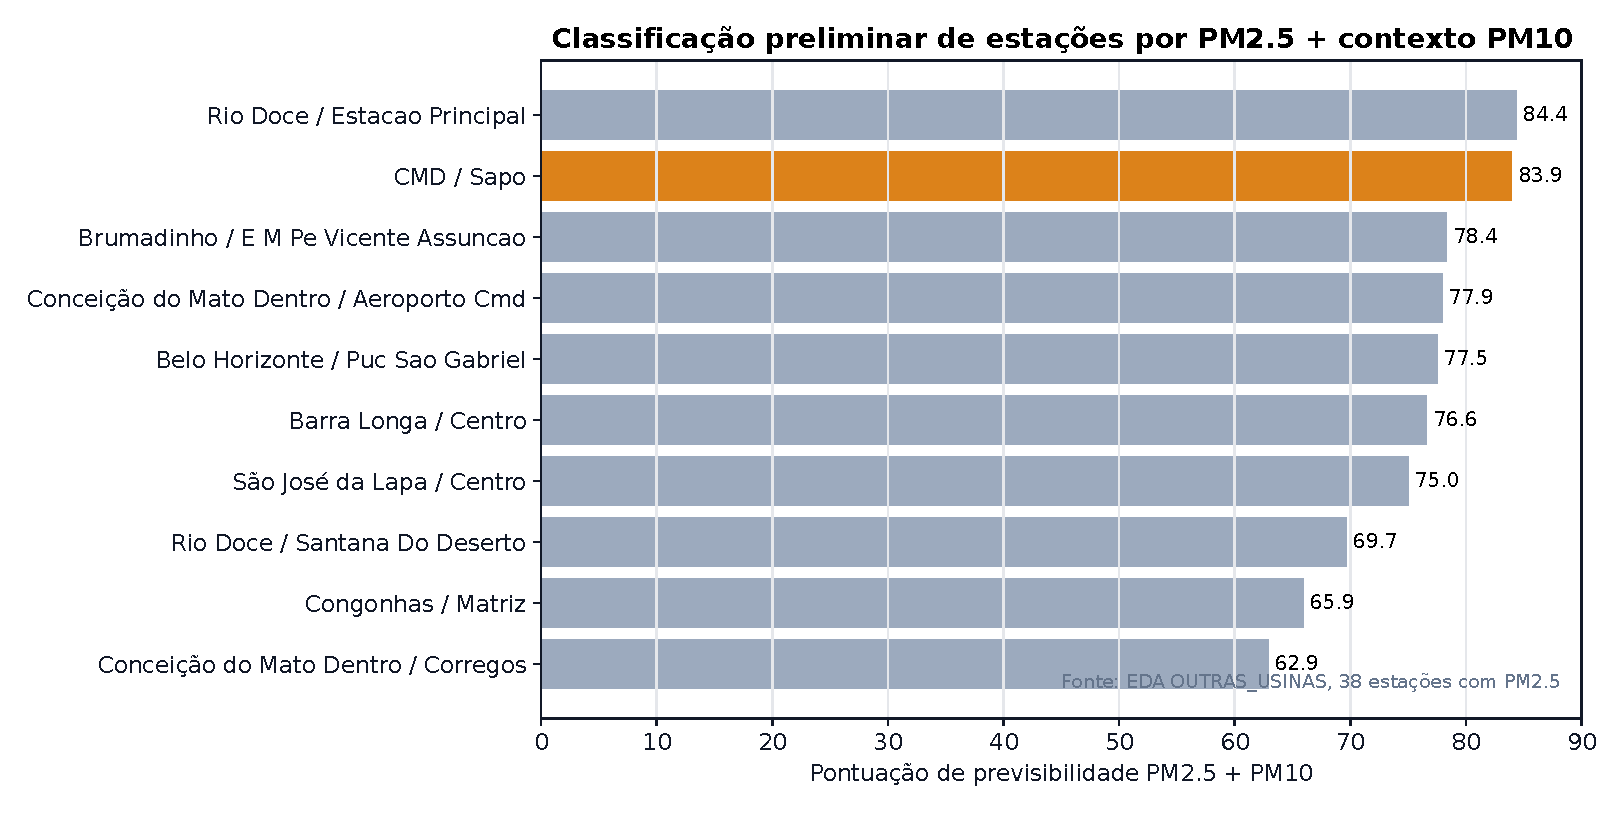
\includegraphics[width=\linewidth]{eda_ranking_estacoes_pm25_pm10.pdf}
    \caption{Classificação preliminar das estações por previsibilidade de PM2,5 com contexto de PM10.}
    \label{fig:eda_ranking_estacoes_pm25_pm10}
\end{figure}

Após a escolha da estação, a análise exploratória foi refeita sobre o conjunto final usado na comparação principal. A Figura \ref{fig:eda_sapo_cobertura_lacunas} mostra que a série não é integralmente contínua: há meses com cobertura elevada, mas também lacunas longas, principalmente na validação. A maior lacuna original de PM2,5 ocorre de 2019-12-11 13:30 a 2020-01-28 18:30, com 48,25 dias, seguida por lacunas de 14,38 dias e 10,83 dias no treino. Por outro lado, ainda existem trechos observados contínuos suficientes para análise de janelas; os maiores blocos contínuos identificados têm cerca de 8,54 dias no treino e 8,13 dias no teste. Esse padrão fundamenta duas decisões metodológicas: manter a série em grade horária regular por interpolação e preservar máscaras de ausência para que valores originalmente imputados não sejam tratados como verdade observada na função de perda nem nas métricas.

\begin{figure}[htb]
    \centering
    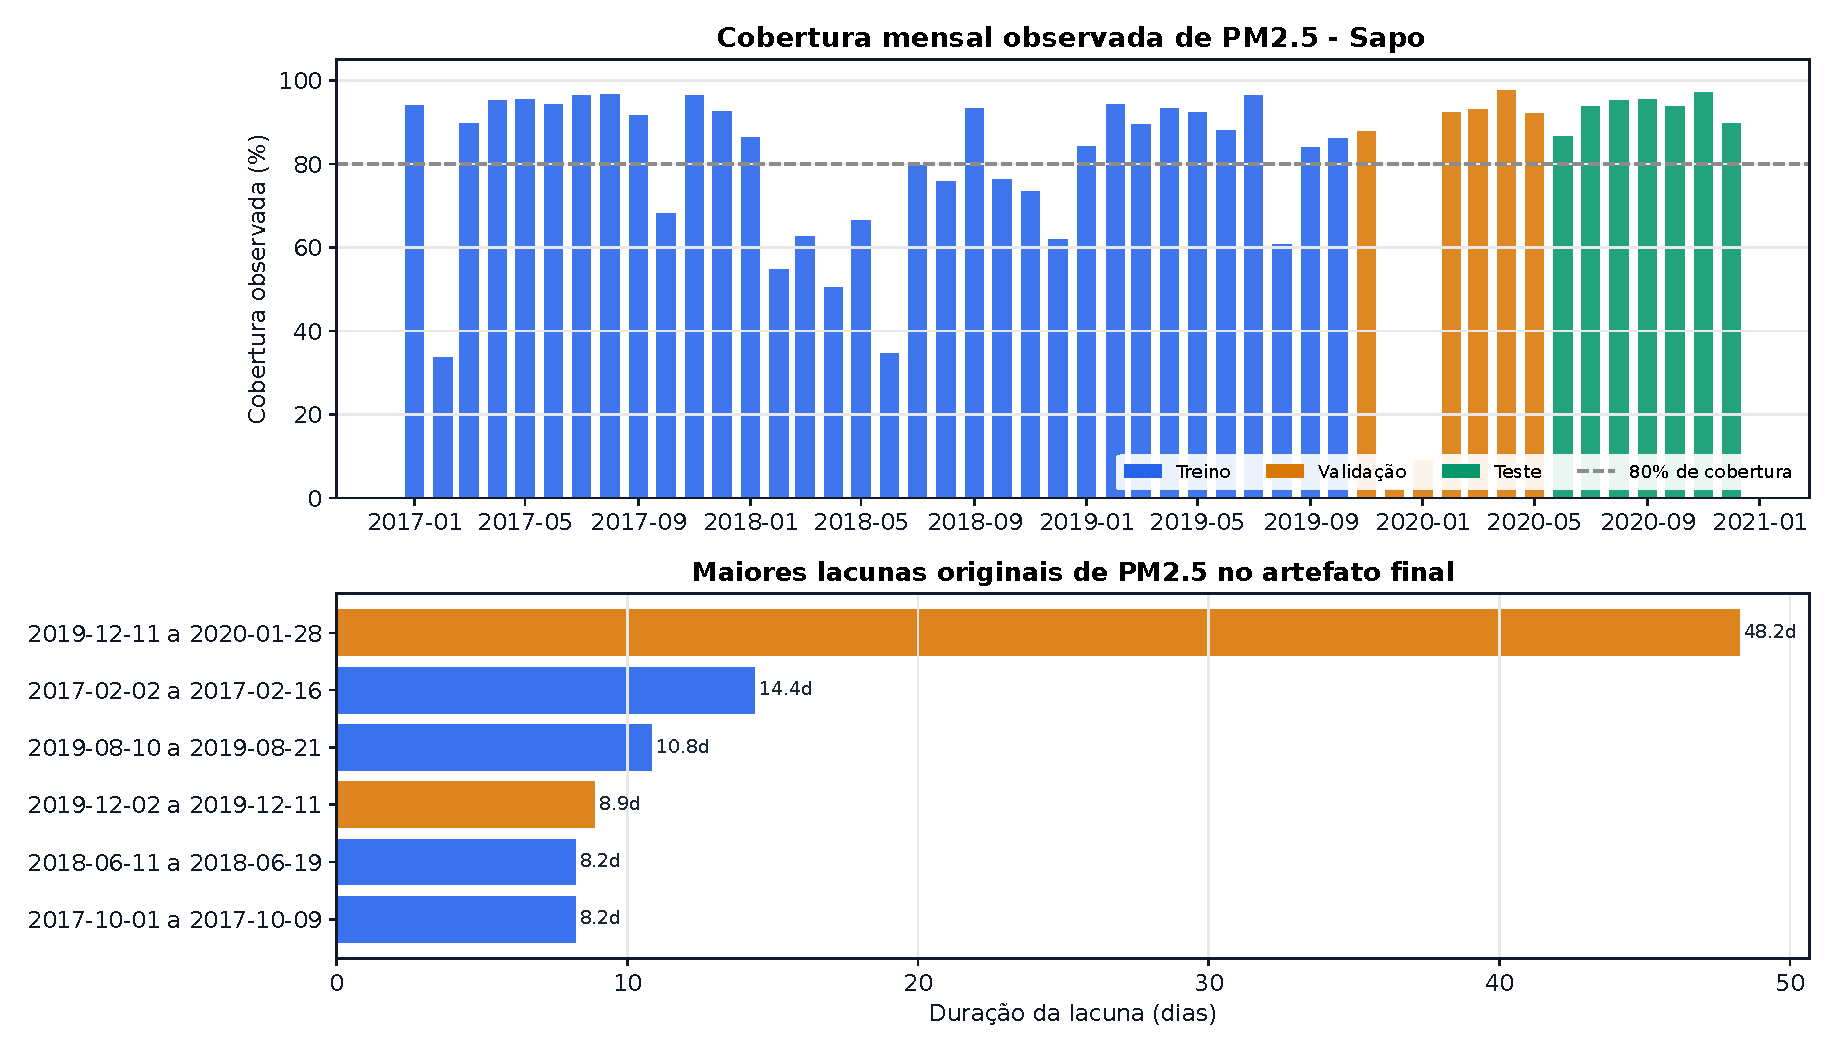
\includegraphics[width=\linewidth]{eda_sapo_cobertura_lacunas.pdf}
    \caption{Cobertura mensal e maiores lacunas originais de PM2,5 no artefato Sapo.}
    \label{fig:eda_sapo_cobertura_lacunas}
\end{figure}

A Tabela \ref{tab:eda_sapo_splits} resume a cobertura e a distribuição observada por partição. O teste apresenta a maior cobertura observada de PM2,5 (93,37\%), enquanto a validação concentra a maior proporção de ausências (31,73\%). A distribuição também mostra que os eventos altos são raros em todas as partições: 1,57\% dos pontos observados no treino, 1,45\% na validação e 0,96\% no teste ficam em PM2,5 \(\geq 35\). Essa raridade justifica a análise de cauda no Capítulo \ref{chap:resultados}, pois o MAE global sozinho tende a privilegiar o regime mais frequente e pode esconder suavização em eventos de maior concentração.

\begin{table}[htb]
    \centering
    \caption{Resumo exploratório do artefato Sapo por partição.}
    \label{tab:eda_sapo_splits}
    \resizebox{\textwidth}{!}{%
    \begin{tabular}{lrrrrrr}
        \toprule
        \textbf{Partição} & \textbf{Cobertura PM2,5} & \textbf{Cobertura PM10} & \textbf{Mediana PM2,5} & \textbf{p95} & \textbf{p99} & \textbf{PM2,5 \(\geq 35\)} \\
        \midrule
        Treino & 80,70\% & 81,33\% & 9,00 & 24,00 & 40,00 & 1,57\% \\
        Validação & 68,27\% & 64,50\% & 12,00 & 25,00 & 37,00 & 1,45\% \\
        Teste & 93,37\% & 92,11\% & 12,00 & 24,00 & 34,00 & 0,96\% \\
        \bottomrule
    \end{tabular}%
    }
\end{table}

\begin{figure}[htb]
    \centering
    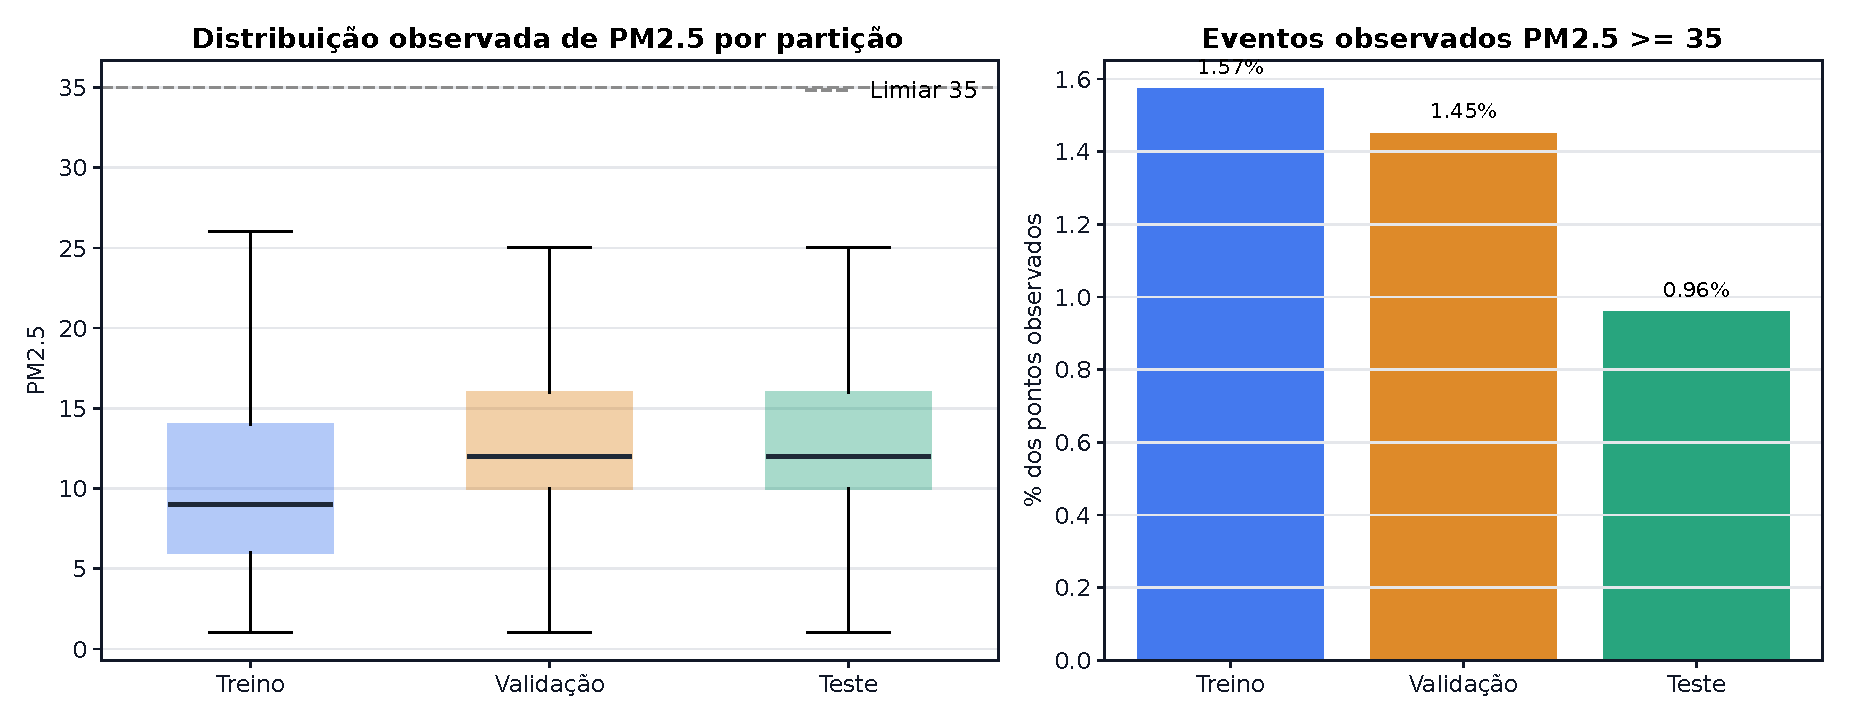
\includegraphics[width=0.95\linewidth]{eda_sapo_distribuicao_pm25.pdf}
    \caption{Distribuição observada de PM2,5 e frequência de eventos altos por partição.}
    \label{fig:eda_sapo_distribuicao_pm25}
\end{figure}

\subsection{Padrões Temporais de PM2,5 e PM10}

Além da cobertura e da distribuição marginal, o artefato Sapo foi analisado quanto a tendência, persistência e sazonalidade. Essa análise usa apenas pontos originalmente observados nas métricas agregadas, respeitando as máscaras \texttt{PM2,5\_\_miss} e \texttt{PM10\_\_miss}. A Figura \ref{fig:serie_temporal_componentes_sapo} resume visualmente a decomposição descritiva do PM2,5: há uma componente lenta de tendência-ciclo, um perfil horário repetitivo e resíduos com picos abruptos.

\begin{figure}[htb]
    \centering
    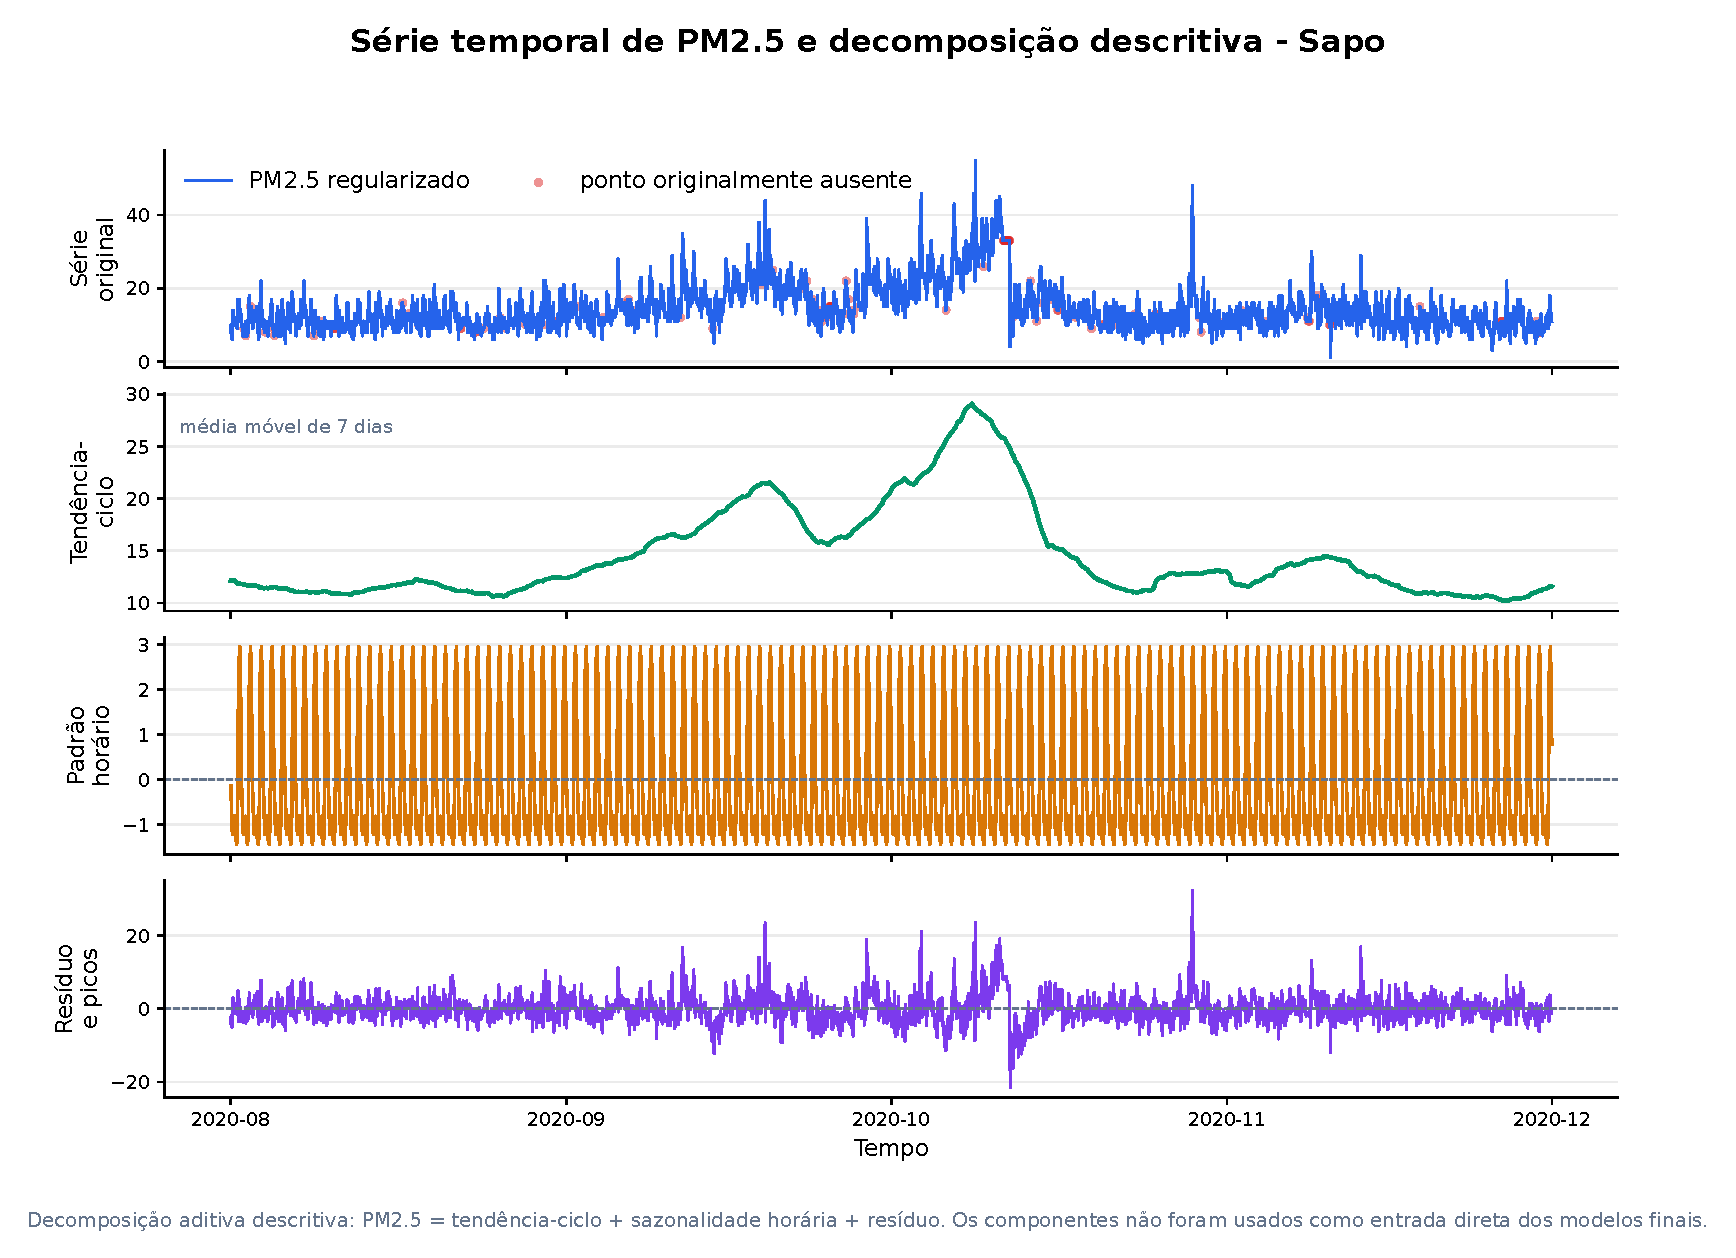
\includegraphics[width=\linewidth]{serie_temporal_componentes_sapo.pdf}
    \caption{Série temporal de PM2,5 e decomposição descritiva no artefato Sapo. Elaboração própria com base na decomposição aditiva discutida por \citeonline{hyndman2021forecasting}.}
    \label{fig:serie_temporal_componentes_sapo}
\end{figure}

A Tabela \ref{tab:padroes_temporais_sapo} resume os principais sinais temporais de PM2,5 e PM10. Para PM2,5, a persistência de curto prazo é alta, com autocorrelação de 0,813 em 1 hora, e há repetição diária relevante, com autocorrelação de 0,681 em 24 horas. O sinal semanal existe, mas é mais fraco, com autocorrelação de 0,461 em 168 horas e diferença média entre dias da semana de apenas 0,70. O perfil horário é mais claro: as menores médias de PM2,5 aparecem entre a madrugada e o início da tarde, com mínimo médio próximo de 10,29 às 13h, enquanto o fim da tarde e a noite concentram maiores valores, com máximo médio próximo de 14,77 às 18h.

\begin{table}[htb]
    \centering
    \caption{Padrões temporais observados de PM2,5 e PM10 no artefato Sapo.}
    \label{tab:padroes_temporais_sapo}
    \resizebox{\textwidth}{!}{%
    \begin{tabular}{lrrp{0.44\textwidth}}
        \toprule
        \textbf{Diagnóstico} & \textbf{PM2,5} & \textbf{PM10} & \textbf{Leitura} \\
        \midrule
        Autocorrelação 1h & 0,813 & 0,734 & Forte persistência de curto prazo nos dois poluentes. \\
        Autocorrelação 24h & 0,681 & 0,564 & Repetição diária relevante, justificando defasagens e substitutos causais baseados em 24h. \\
        Autocorrelação 168h & 0,461 & 0,360 & Sinal semanal mais fraco que o diário. \\
        Amplitude média por hora & 4,48 & 11,14 & Ciclo horário claro, mais intenso em PM10. \\
        Amplitude média por dia da semana & 0,70 & 3,68 & Variação semanal pequena diante da variabilidade total. \\
        Amplitude média por mês & 8,52 & 12,95 & Regime sazonal/mensal forte, com elevação em setembro e outubro. \\
        \bottomrule
    \end{tabular}%
    }
\end{table}

O PM10 apresenta comportamento compatível com o PM2,5, mas com amplitude horária maior. Suas menores médias ocorrem por volta de 4h, com valor médio próximo de 20,95, e as maiores médias ocorrem por volta de 20h, com valor médio próximo de 32,09. A correlação de Pearson entre PM2,5 e PM10 observados no mesmo horário foi 0,597, e a correlação de Spearman foi 0,421. Portanto, PM10 é uma variável auxiliar informativa, mas não determina completamente a variação horária de PM2,5.

Também há um padrão mensal importante: PM2,5 e PM10 sobem em setembro e outubro, com média de PM2,5 próxima de 17,97 em outubro e p95 de 44 nesse mês. No entanto, a interpretação como ciclo anual regular deve ser cautelosa, pois o artefato cobre apenas quatro anos, possui lacunas e apresenta mudanças de regime entre anos. A autocorrelação anual aproximada de PM2,5 foi baixa, cerca de 0,038, indicando que a repetição anual é menos estável que a persistência horária e diária. Assim, no protocolo final, os termos temporais e de Fourier são úteis para fornecer informação cíclica ao modelo, mas os picos e resíduos continuam dependendo de fatores não observados diretamente, como meteorologia local, mistura atmosférica, transporte espacial e fontes de emissão.

\clearpage

\section{Formulação da Tarefa}

A tarefa de previsão é multi-horizonte: para cada janela válida, os modelos recebem as 48 horas anteriores e produzem uma previsão para as 24 horas seguintes. Formalmente, para um instante inicial \(t\), a entrada contém observações de \(t-47\) até \(t\), e a saída corresponde aos horizontes \(t+1\) até \(t+24\). Essa formulação foi mantida para todos os modelos da comparação principal e está resumida na Figura \ref{fig:tarefa_48_24_sapo}.

Essa escolha de 48 horas foi reavaliada por uma análise auxiliar de persistência no próprio artefato final de Sapo. A autocorrelação observada de PM2,5 foi alta em uma hora (\(0{,}813\)) e ainda relevante em 24 horas (\(0{,}681\)), confirmando que o ciclo diário carrega informação importante para a previsão. Em 48 horas, a autocorrelação permaneceu moderada (\(0{,}598\)), enquanto o sinal semanal de 168 horas foi mais fraco (\(0{,}461\)). Além disso, linhas de base e modelos lineares diagnósticos com janelas de 1 a 168 horas indicaram que a maior parte do ganho ocorre ao cobrir as primeiras 24 horas, sem melhora consistente ao ampliar a entrada para uma semana completa. Assim, a janela de 48 horas foi mantida como compromisso metodológico: ela preserva dois ciclos diários, permite comparar defasagens de 24 e 48 horas e mantém custo computacional controlado, mas não deve ser interpretada como evidência de que históricos mais longos sejam sempre desnecessários em outros recortes.

\begin{figure}[htb]
    \centering
    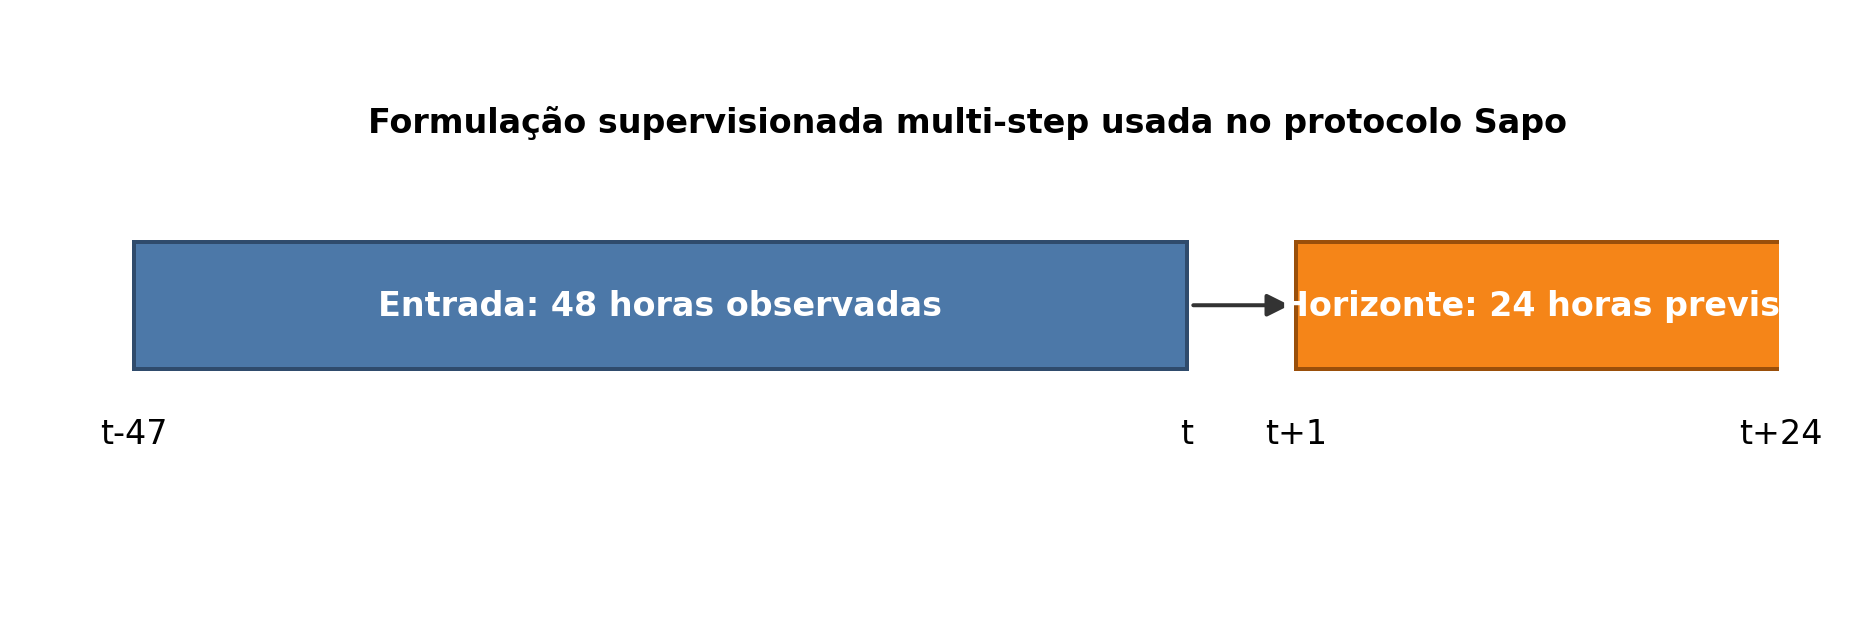
\includegraphics[width=0.95\linewidth]{tarefa_48_24_sapo.png}
    \caption{Formulação da tarefa 48 para 24 horas do protocolo Sapo.}
    \label{fig:tarefa_48_24_sapo}
\end{figure}

A divisão do conjunto de dados é cronológica e usa 70\% dos horários para treino final, 15\% para validação de treinamento e 15\% para teste final. A Tabela \ref{tab:split_temporal_sapo} apresenta os limites reais do artefato final, e a Figura \ref{fig:split_70_15_15_sapo} mostra a mesma divisão na linha do tempo. O conjunto de teste contém os horários mais recentes e só é usado para avaliação final.

\begin{table}[htb]
    \centering
    \caption{Divisão cronológica externa do conjunto final de Sapo.}
    \label{tab:split_temporal_sapo}
    \begin{tabular}{lrrl}
        \toprule
        \textbf{Partição} & \textbf{Proporção} & \textbf{Timestamps} & \textbf{Intervalo} \\
        \midrule
        Treino & 70\% & 24.495 & 2017-01-04 00:30 a 2019-10-21 14:30 \\
        Validação & 15\% & 5.248 & 2019-10-21 15:30 a 2020-05-27 06:30 \\
        Teste & 15\% & 5.248 & 2020-05-27 07:30 a 2020-12-31 22:30 \\
        \bottomrule
    \end{tabular}
\end{table}

\begin{figure}[htb]
    \centering
    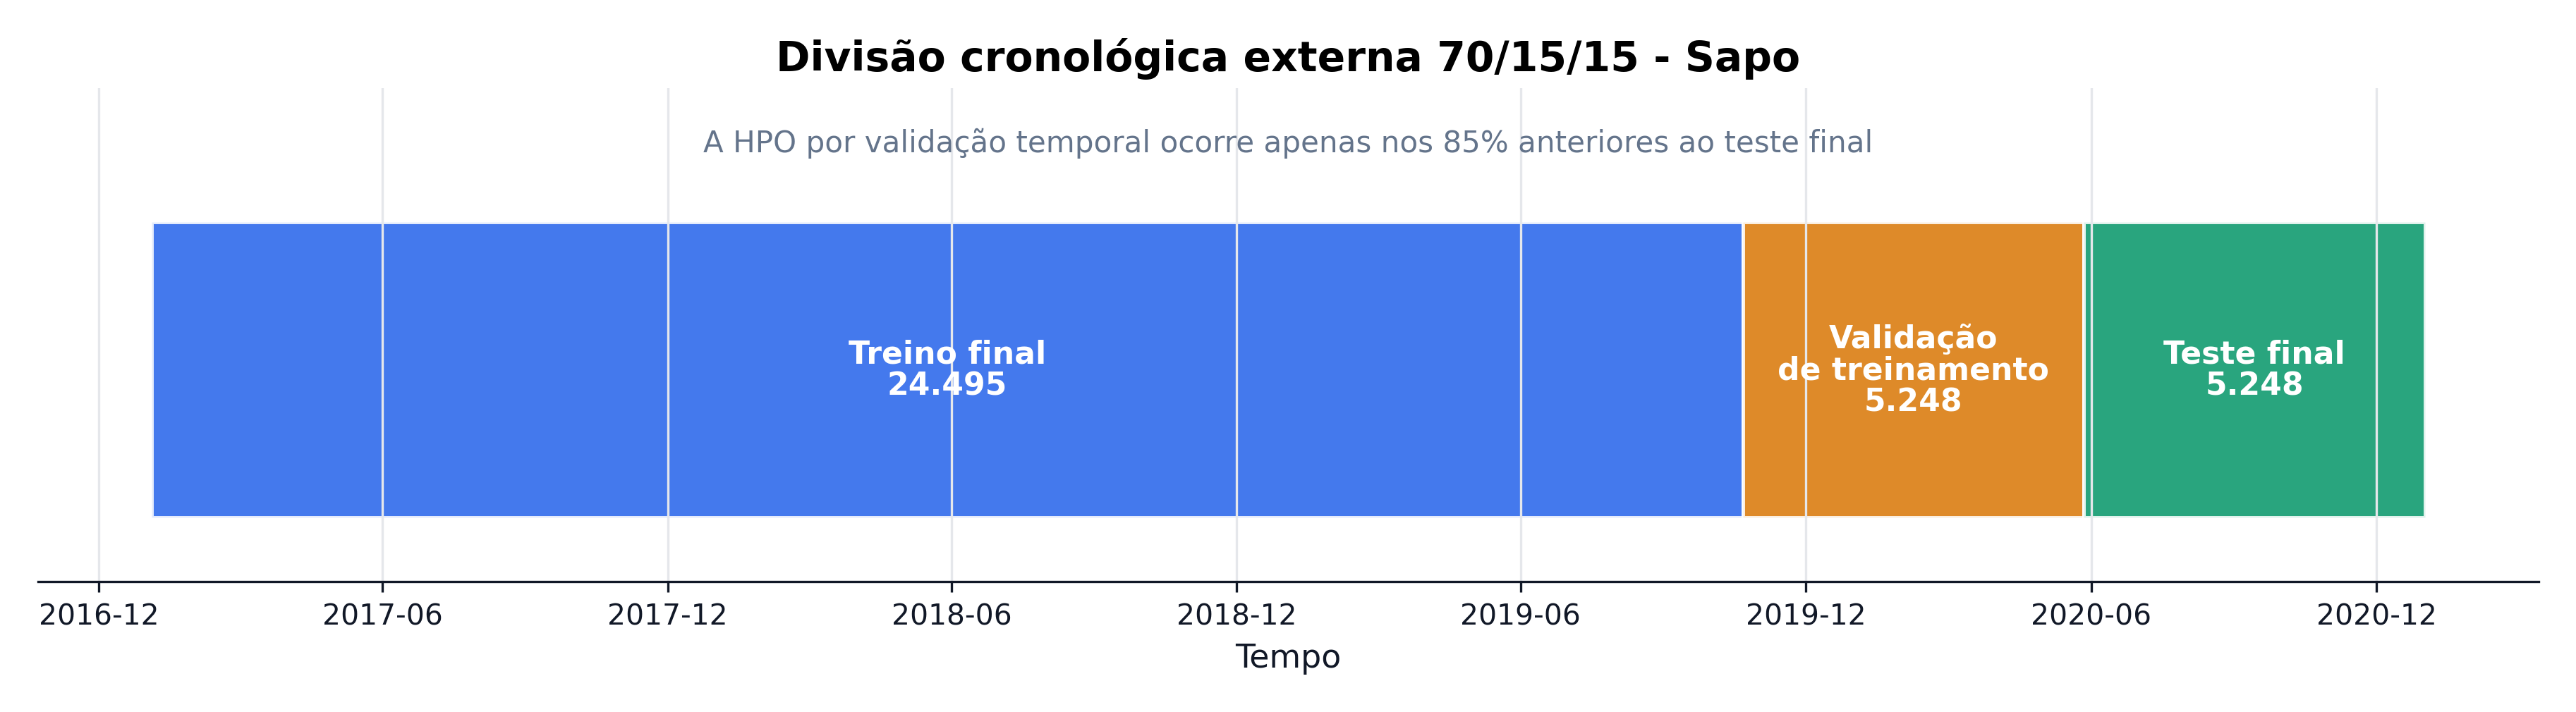
\includegraphics[width=\linewidth]{split_70_15_15_sapo.png}
    \caption{Linha temporal da divisão cronológica usada no artefato Sapo.}
    \label{fig:split_70_15_15_sapo}
\end{figure}

Neste relatório, portanto, a expressão 70/15/15 se refere à divisão cronológica de avaliação. A seleção de hiperparâmetros não usa o teste final: ela é feita por \textit{walk-forward} dentro dos 85\% anteriores ao teste. Em seguida, os modelos selecionados são treinados no protocolo final usando o trecho de treino e a validação de treinamento para parada antecipada e escolha de ponto de controle. A validação intermediária faz parte do desenvolvimento do modelo; o único conjunto tratado como avaliação independente é o teste final.

\section{Pré-processamento}

O pré-processamento foi desenhado para reduzir vazamento temporal. A imputação é ajustada sobre o trecho de treino e aplicada ao restante do período respeitando a separação temporal. No contrato final, usa-se interpolação linear no bloco de treino; para o bloco posterior ao fim do treino, a transformação não usa âncoras futuras e propaga o último estado imputado disponível. Para cada variável imputada, é mantido um indicador \texttt{\_\_miss}, que informa se o valor original estava ausente.

O alvo PM2,5 também possui uma máscara de observação. Quando essa máscara está disponível, pontos do alvo originalmente imputados são excluídos da função de perda e das métricas observadas, seguindo a distinção entre valor observado e valor ausente ou estimado discutida na literatura de dados faltantes e imputação temporal \cite{rubin1976inference,cao2018brits,du2023saits}. Assim, o modelo pode receber uma série regularizada para formar janelas, mas não é recompensado por prever como ``verdade'' um valor que foi produzido pelo próprio pré-processamento.

A normalização é calculada com estatísticas do conjunto de treino. No treinamento dos modelos neurais, médias e desvios são computados por estação e aplicados às janelas de treino, validação e teste. Essa decisão evita que informação agregada dos períodos de validação e teste entre no ajuste de escala do modelo.

\section{Engenharia de Atributos}

O conjunto final de atributos foi mantido enxuto. O codificador recebe PM2,5, PM10, indicadores de ausência e atributos temporais. O decodificador dos modelos que aceitam entradas futuras recebe apenas variáveis conhecidas causalmente no momento da previsão: termos temporais/Fourier e substitutos derivados de PM10. A Tabela \ref{tab:variaveis_contrato} resume os grupos de variáveis.

\begin{table}[htb]
    \centering
    \caption{Variáveis do protocolo final.}
    \label{tab:variaveis_contrato}
    \resizebox{\textwidth}{!}{%
    \begin{tabular}{lll}
        \toprule
        \textbf{Grupo} & \textbf{Variáveis} & \textbf{Uso} \\
        \midrule
        Alvo e histórico & \texttt{PM2,5} & Entrada histórica e alvo da previsão \\
        Poluente auxiliar & \texttt{PM10} & Entrada histórica no codificador \\
        Ausência & \texttt{PM2,5\_\_miss}, \texttt{PM10\_\_miss} & Indicar valores originalmente ausentes \\
        Tempo & \texttt{hour}, \texttt{day\_of\_week}, \texttt{month} & Sazonalidade discreta \\
        Fourier & termos seno/cosseno de 6h, 12h, 24h, 168h e 8760h & Sazonalidade cíclica \\
        Substituto PM10 & \texttt{PM10\_proxy\_exante} & PM10 do mesmo horário no dia anterior, isto é, PM10(t-24) \\
        Tendência PM10 & \texttt{PM10\_trend\_exante} & Diferença causal PM10(t-24) - PM10(t-27) \\
        \bottomrule
    \end{tabular}%
    }
\end{table}

O uso de PM10 no decodificador não assume conhecimento futuro de PM10 observado. O substituto causal usa o valor defasado em 24 horas, e a tendência causal usa a diferença entre valores também defasados. Portanto, ambas podem ser calculadas no instante de emissão da previsão. Variáveis meteorológicas e gases muito esparsos foram excluídos do contrato principal; sua reintrodução deve ser tratada apenas como nova ablação, não como parte da comparação final.

\section{Modelos Avaliados}

Foram comparadas cinco variantes neurais e um modelo de referência baseado em árvores. A Tabela \ref{tab:modelos_metodologia} resume o papel de cada modelo no desenho experimental.

\begin{table}[htb]
    \centering
    \caption{Modelos avaliados na comparação principal.}
    \label{tab:modelos_metodologia}
    \resizebox{\textwidth}{!}{%
    \begin{tabular}{lll}
        \toprule
        \textbf{Modelo} & \textbf{Descrição} & \textbf{Papel na comparação} \\
        \midrule
        LSTM recursiva & Prevê passo a passo, realimentando a trajetória prevista & Linha de base sequencial recursiva \\
        LSTM direta & Produz os 24 horizontes de uma vez & Modelo sequencial direto \\
        Seq2Seq básico & Codificador-decodificador recorrente sem atenção explícita & Linha de base codificador-decodificador \\
        Seq2Seq atenção canônica & Codificador-decodificador com mecanismo de atenção e perda Huber & Variante de referência para análise de atenção \\
        Seq2Seq atenção novo & Codificador-decodificador com atenção, perda ponderada, reinício do decodificador e agrupamento por defasagens & Variante final de Seq2Seq \\
        XGBoost com saída múltipla & Árvores com saída multi-horizonte & Referência baseada em árvores sobre atributos de janelas \\
        \bottomrule
    \end{tabular}%
    }
\end{table}

A escolha dos modelos também delimita o escopo do estudo. Transformers temporais, como o \textit{Temporal Fusion Transformer} (TFT), Informer, Autoformer e PatchTST, são alternativas modernas para previsão multi-horizonte \cite{lim2021tft,zhou2021informer,wu2021autoformer,nie2023patchtst}. Eles não foram incluídos na comparação final porque uma comparação justa exigiria nova família de arquitetura, espaço próprio de hiperparâmetros, orçamento adicional de otimização de hiperparâmetros (HPO), avaliação com múltiplas sementes e decisões específicas de regularização para o tamanho e a qualidade do conjunto de dados Sapo. Além disso, a literatura não autoriza assumir que Transformers vencem automaticamente em séries temporais; \citeonline{zeng2023transformers} mostram que linhas de base simples podem superar Transformers em alguns cenários de previsão. Assim, o recorte deste TCC é comparar famílias recorrentes e modelos baseados em atributos derivados das janelas temporais sob um contrato causal rastreável, deixando Transformers como extensão natural para trabalhos futuros.

A comparação com XGBoost exige uma ressalva metodológica. O modelo de referência baseado em árvores usa o mesmo contrato causal de entrada e é avaliado no mesmo bloco final de teste, mas seu treinamento com saída múltipla exige janelas com horizonte completo observado. Nos modelos neurais, a máscara de alvo observado permite ignorar pontos imputados da função de perda e das métricas. Assim, a avaliação de teste é comparável, mas o mecanismo de treino não é perfeitamente simétrico.

Além da comparação principal, foram executados experimentos diagnósticos com o Seq2Seq atenção para investigar limites informacionais do problema. O primeiro é o \textit{oracle future auxiliary}: no decodificador, o modelo recebe PM10 e partículas totais em suspensão (PTS) reais do próprio horizonte futuro. Esse cenário não representa um uso causal de previsão, pois usa informação indisponível no instante de previsão, mas mede quanto desempenho poderia ser recuperado caso variáveis auxiliares futuras relevantes fossem conhecidas. O segundo é o Seq2Seq multi-alvo, no qual a rede continua prevendo PM2,5 como alvo principal, mas recebe uma cabeça auxiliar para prever PM10 e PTS futuros durante o treinamento. Esse teste avalia se aprender variáveis correlacionadas em conjunto ajuda a representação interna sem introduzir vazamento na avaliação causal.

Esses dois experimentos não substituem o protocolo final nem entram como candidatos a vencedor, porque usam contratos diferentes do contrato causal principal. Eles são apresentados nos resultados como análise de limite: o \textit{oracle} mostra o ganho máximo associado a variáveis futuras observadas, enquanto o multi-alvo testa se a própria arquitetura consegue aproximar esse ganho apenas aprendendo as auxiliares.

\section{Treinamento e Busca de Hiperparâmetros}

O resultado principal usa hiperparâmetros selecionados no bloco de desenvolvimento anterior ao teste. Para LSTM direta, LSTM recursiva e XGBoost, a seleção foi feita por validação temporal \textit{walk-forward}. Para os modelos neurais principais com HPO, foram usadas 24 tentativas, três partições temporais por janela expansiva, até 18 épocas por tentativa e treinamento final de até 36 épocas para LSTM direta e LSTM recursiva. Para o novo Seq2Seq atenção, a configuração final veio de ablações focadas em arquitetura, perda, resposta a picos e tamanho de janela, e foi reexecutada no mesmo protocolo final com quatro sementes. O XGBoost foi submetido ao mesmo desenho \textit{walk-forward}, mas, por custo computacional das tentativas mais longas, o resultado consolidado usou quatro tentativas completas.

Nas redes neurais, cada tentativa reiniciou o modelo em cada partição e agregou a métrica de validação ao fim das partições. O estudo do Optuna usou o amostrador padrão \texttt{TPESampler} e o \texttt{HyperbandPruner}, com \texttt{min\_resource}=1, \texttt{max\_resource}=18 e fator de redução 3. Assim, tentativas pouco promissoras podiam ser interrompidas antes de consumir todo o orçamento de épocas. Essa escolha segue a recomendação da documentação do Optuna para a combinação entre \texttt{TPESampler} e \texttt{HyperbandPruner} \cite{optunaDocsEfficient2026,optunaDocsHyperband2026}. Para o XGBoost, a busca minimizou o MAE médio nas partições, com parada antecipada (\textit{early stopping}) nativa do XGBoost e \texttt{MedianPruner} \cite{optunaDocsMedian2026}. A Tabela \ref{tab:hpo_espaco_busca} organiza o espaço de busca por grupo de hiperparâmetros; a Tabela \ref{tab:hpo_melhores_hiperparametros} apresenta a configuração selecionada.

Nos modelos neurais, a taxa de aprendizado apresentada nas tabelas é a taxa nominal \(\eta_{\max}\) escolhida pela HPO. As execuções finais usaram AdamW com agenda ativa por época: três épocas de aquecimento linear, saindo de \(10^{-5}\eta_{\max}\) até \(\eta_{\max}\), seguidas de decaimento cosseno até \(0{,}01\eta_{\max}\) no fim do orçamento. A agenda é reiniciada em cada partição da HPO e em cada treinamento final. A validação ao fim das épocas monitora MAE para poda, parada antecipada e escolha do melhor \textit{checkpoint}, mas não recalcula a taxa de aprendizado com base no valor da métrica.

\begin{table}[htb]
    \centering
    \caption{Espaço de busca e configuração selecionada na comparação principal.}
    \label{tab:hpo_espaco_busca}
    \small
    \renewcommand{\arraystretch}{1.08}
    \begin{tabular}{>{\raggedright\arraybackslash}p{0.19\textwidth}>{\raggedright\arraybackslash}p{0.23\textwidth}>{\raggedright\arraybackslash}p{0.48\textwidth}}
        \toprule
        \textbf{Grupo} & \textbf{Hiperparâmetro} & \textbf{Valores avaliados} \\
        \midrule
        Redes neurais & Taxa nominal de aprendizado & 0{,}0003; 0{,}0005; 0{,}0008; 0{,}0012; 0{,}0018; 0{,}0025; 0{,}0035; 0{,}005; 0{,}007 \\
        Redes neurais & Decaimento de pesos & 0; $10^{-7}$; $5 \times 10^{-7}$; $10^{-6}$; $5 \times 10^{-6}$; $10^{-5}$; $5 \times 10^{-5}$; $10^{-4}$ \\
        Redes neurais & Taxa de \textit{dropout} & 0{,}00; 0{,}05; 0{,}10; 0{,}15; 0{,}20; 0{,}25; 0{,}30 \\
        Redes neurais & Profundidade e perda & número de camadas 1; 2; 3; $\delta$ da Huber em 0{,}5; 0{,}75; 1{,}0; 1{,}5; 2{,}0 \\
        LSTM direta & Arquitetura & dimensão oculta 96; 128; 192; 256; 320; agregação por último estado, média ou atenção \\
        LSTM recursiva & Arquitetura & dimensão oculta 96; 128; 192; 256; 320 \\
        Seq2Seq atenção novo & Arquitetura e perda & variante selecionada por ablações: codificador/decodificador 96; uma camada; atenção de entrada 96; representação de horizonte 24; reinício do decodificador por horizonte; sem \textit{input feeding}; atenção por \textit{lag buckets}; perda ponderada e perda auxiliar leve de evento \\
        XGBoost com saída múltipla & Árvores e profundidade & 160; 240; 320; 480 árvores; profundidade máxima 2 a 7; \texttt{max\_bin} 64; 128; 256 \\
        XGBoost com saída múltipla & Regularização, amostragem e parada & taxa de aprendizado logarítmica entre 0{,}015 e 0{,}12; \textit{subsample} e \textit{colsample} entre 0{,}60 e 1{,}0; $\lambda$, $\alpha$, $\gamma$, peso mínimo do filho (\textit{min child weight}); parada antecipada (\textit{early stopping}) de 10, 15 ou 25 rodadas \\
        \bottomrule
    \end{tabular}
\end{table}

\begin{table}[htb]
    \centering
    \caption{Hiperparâmetros e configurações selecionadas na comparação principal.}
    \label{tab:hpo_melhores_hiperparametros}
    \small
    \renewcommand{\arraystretch}{1.08}
    \begin{tabular}{>{\raggedright\arraybackslash}p{0.20\textwidth}>{\raggedright\arraybackslash}p{0.35\textwidth}>{\raggedright\arraybackslash}p{0.35\textwidth}}
        \toprule
        \textbf{Modelo} & \textbf{Arquitetura selecionada} & \textbf{Treinamento e regularização} \\
        \midrule
        LSTM direta & dimensão oculta 256; 3 camadas; agregação por média & taxa nominal de aprendizado 0{,}007; decaimento de pesos $5 \times 10^{-5}$; \textit{dropout} 0{,}20; $\delta$ da Huber 2{,}0 \\
        LSTM recursiva & dimensão oculta 128; 2 camadas & taxa nominal de aprendizado 0{,}0035; decaimento de pesos 0; \textit{dropout} 0{,}20; $\delta$ da Huber 1{,}0 \\
        Seq2Seq atenção novo & codificador 96; decodificador 96; 1 camada; atenção de entrada 96; representação de horizonte 24; \textit{lag buckets} com janela 2 & taxa nominal de aprendizado 0{,}005; decaimento de pesos $10^{-6}$; \textit{dropout} 0{,}25; pesos 1{,}05/1{,}10; fator de subestimação 1{,}50; perda auxiliar de evento 0{,}035 \\
        XGBoost com saída múltipla & 480 árvores; profundidade máxima 2; \texttt{max\_bin}=64 & taxa de aprendizado 0{,}02563; \textit{subsample}=0{,}7611; \textit{colsample}=0{,}9073; $\lambda=7{,}7542$; parada antecipada=10 rodadas \\
        \bottomrule
    \end{tabular}
\end{table}

\clearpage

A formulação final do Seq2Seq priorizou a nova variante com atenção de entrada, perda \texttt{weighted\_l1}, reinício do estado do decodificador a cada horizonte, remoção de \textit{input feeding}, atenção condicionada por horizonte e variáveis do decodificador, agrupamento por \textit{lag buckets} e perda auxiliar leve para eventos. A perda pondera regimes de concentração e tipos de erro, alterando o objetivo de treinamento para reduzir parte da suavização e melhorar o comportamento em concentrações mais altas. Essa variante foi avaliada no protocolo consolidado com múltiplas sementes e janela fixa de 48 horas, após ablações indicarem que janelas de 72, 96 e 168 horas não traziam ganho claro.

As variantes finais de Seq2Seq priorizaram um decodificador semidireto com horizonte explícito e linha de base residual sazonal, reduzindo a dependência de realimentação autoregressiva pura. Ainda assim, a avaliação de agendas de \textit{teacher forcing} foi incluída porque trabalhos recentes em previsão, como \citeonline{teutsch2022flipped}, indicam que currículos crescentes de \textit{teacher forcing} podem melhorar previsões multi-horizonte em séries temporais contínuas. No relatório, portanto, \textit{teacher forcing} e \textit{scheduled sampling} são tratados como técnicas avaliadas em ablações auxiliares fundamentadas, não como eixo central do resultado final em Sapo. Essa distinção evita atribuir ao \textit{scheduled sampling} um ganho que, nos experimentos consolidados, esteve mais associado ao contrato de dados, ao uso causal de PM10, à seleção por validação e à função de perda.

\section{Métricas de Avaliação}

A avaliação final utiliza métricas no bloco final de teste. As métricas globais principais são erro médio absoluto (MAE), raiz do erro quadrático médio (RMSE), erro percentual médio absoluto (MAPE) e coeficiente de determinação (\(R^2\)). Também são reportadas métricas por horizonte, especialmente nos horizontes 1, 6, 12 e 24, para observar degradação ao longo da previsão; os rótulos H1, H6, H12 e H24 indicam esses horizontes em horas. Como os picos são raros e importantes em qualidade do ar, a análise também considera métricas de cauda, como erro em eventos acima de 35, percentil 99 previsto (p99), razão entre desvio-padrão previsto e observado, viés médio medido pelo erro médio de viés (\textit{Mean Bias Error}, MBE) e taxa de subestimação. Nas tabelas, o rótulo Peak35 MAE indica o MAE calculado em pontos ou eventos com PM2,5 \(\geq 35\).

A interpretação dos resultados combina métricas agregadas e inspeção visual das séries previstas. Essa combinação é necessária porque modelos que vencem em erro médio podem produzir previsões mais suaves, enquanto variantes voltadas a picos podem preservar mais amplitude ao custo de pequeno aumento no MAE global.

\section{Reprodutibilidade}

A reprodutibilidade foi tratada por meio de scripts determinísticos de geração de figuras, tabelas e diagnósticos, mantendo a separação entre treino, validação e teste. Os experimentos principais foram executados com identificadores de execução, sementes registradas quando aplicável, configuração explícita de HPO e exportação de métricas em arquivos estruturados. No corpo do TCC, os valores reportados são apresentados diretamente nas tabelas e nas figuras; os caminhos técnicos e hashes dos arquivos ficam preservados como material de controle do projeto, sem substituir a descrição metodológica.

% cap_resultados.tex
\chapter{Resultados e Discussão}
\label{chap:resultados}

Este capítulo apresenta os resultados do protocolo Sapo descrito no Capítulo \ref{chap:materiais_metodos}. A discussão separa quatro níveis de evidência: a comparação principal com hiperparâmetros selecionados no bloco de desenvolvimento, a estabilidade com múltiplas sementes dos modelos selecionados, as linhas de base ingênuas e as ablações usadas para interpretar decisões de modelagem.

As métricas usadas no capítulo seguem as definições da Seção \ref{sec:metricas_avaliacao}: erro médio absoluto (MAE), raiz do erro quadrático médio (RMSE), erro percentual médio absoluto (MAPE), coeficiente de determinação (\(R^2\)), erro médio de viés (MBE) e MAE em eventos com PM2,5 \(\geq 35\) (Peak35 MAE). Em todos os casos, a referência de avaliação é a medição real de PM2,5 disponível no teste.

\section{Caracterização da Comparação Principal}

A comparação principal usa a estação Sapo, tarefa 48 para 24 horas e divisão cronológica 70/15/15. A seleção de hiperparâmetros e ablações ocorre no bloco de desenvolvimento, e a avaliação é feita no bloco final de teste. O conjunto de dados final contém 34.991 registros horários. No conjunto consolidado, a proporção de valores originalmente ausentes é de aproximadamente 19,26\% para material particulado fino (PM2,5) e 19,58\% para material particulado com diâmetro de até 10 micrômetros (PM10). Esses percentuais reforçam a importância de manter indicadores de ausência e de avaliar os modelos contra medições reais disponíveis.

Os eventos altos são raros no teste. Na caracterização exploratória do bloco final, pontos observados com PM2,5 \(\geq 35\) representam cerca de 0,96\% do teste. Portanto, o MAE global é dominado por regimes baixos e moderados. A análise de cauda é apresentada separadamente para evitar que o melhor erro médio seja confundido com melhor resposta a picos.

\section{Resultado Principal no Protocolo Final}

A Tabela \ref{tab:resultado_principal_sapo_hpo} apresenta os resultados principais no bloco final de teste. Todos os modelos foram reexecutados no mesmo contrato final, com 48 horas de entrada, 24 horas de horizonte, conjunto \texttt{clean\_pm10\_decoder\_proxy}, mesma divisão cronológica e as mesmas medições de PM2,5 como referência. As LSTMs e o XGBoost usam hiperparâmetros selecionados por validação temporal \textit{walk-forward}; o novo Seq2Seq atenção usa a variante selecionada pelas ablações de arquitetura, perda e janela de entrada, reexecutada aqui no mesmo protocolo comparável. O melhor desempenho global na semente canônica foi obtido pela LSTM direta, enquanto o novo Seq2Seq atenção ficou em segundo por MAE e apresentou melhor comportamento em picos.

\begin{table}[htb]
    \centering
    \caption{Resultado principal no protocolo final de Sapo.}
    \label{tab:resultado_principal_sapo_hpo}
    \resizebox{\textwidth}{!}{%
    \begin{tabular}{lrrrrrr}
        \toprule
        \textbf{Modelo} & \textbf{MAE} & \textbf{RMSE} & \textbf{MAPE} & \textbf{\(R^2\)} & \textbf{H1 MAE} & \textbf{H24 MAE} \\
        \midrule
        LSTM direta & \textbf{2,7713} & \textbf{3,8346} & \textbf{23,01} & \textbf{0,5154} & 2,6725 & \textbf{2,8670} \\
        Seq2Seq atenção novo & 2,8132 & 3,8799 & 23,23 & 0,5039 & 2,6222 & 2,9138 \\
        XGBoost com saída múltipla & 2,8786 & 3,9793 & 23,80 & 0,4781 & \textbf{2,5618} & 3,0273 \\
        Seq2Seq atenção canônica & 2,8811 & 3,9859 & 23,79 & 0,4764 & 2,7155 & 2,9743 \\
        LSTM recursiva & 2,8876 & 3,8380 & 24,39 & 0,5146 & 2,7380 & 3,1492 \\
        Seq2Seq básico & 2,9553 & 4,0967 & 23,99 & 0,4469 & 2,6519 & 3,1514 \\
        \bottomrule
    \end{tabular}%
    }
\end{table}

O resultado reforça a conclusão central: a LSTM direta permanece vencedora por erro médio. O novo Seq2Seq atenção melhora substancialmente a posição da família Seq2Seq em relação à variante ponderada anterior, reduzindo o MAE da semente canônica de 2,8658 para 2,8132 e aproximando RMSE e \(R^2\) dos valores da LSTM direta. O XGBoost continua sendo uma referência forte baseada em árvores sobre atributos derivados das janelas temporais e manteve o menor erro no primeiro horizonte, mas perdeu para LSTM direta e novo Seq2Seq no MAE global.

Entre os modelos neurais, a diferença entre LSTM direta e novo Seq2Seq é pequena no erro médio, mas não desaparece: 2,7713 contra 2,8132 na semente canônica. A LSTM recursiva apresentou RMSE e \(R^2\) próximos aos da LSTM direta, mas teve pior MAE e maior erro no horizonte final. O Seq2Seq básico e o Seq2Seq atenção canônica ficaram abaixo da nova variante, mostrando que o ganho veio da combinação específica de desenho do decodificador, perda ponderada, agrupamento de atenção por defasagens e seleção da janela de 48 horas, não apenas do uso genérico de uma arquitetura codificador-decodificador.

\section{Estabilidade com Múltiplas Sementes}

A Tabela \ref{tab:multi_seed_sapo} resume a sensibilidade à semente aleatória para os modelos selecionados. A média inclui a semente canônica 42 e três sementes adicionais: 7, 21 e 123.

\begin{table}[htb]
    \centering
    \caption{Estabilidade com múltiplas sementes dos modelos selecionados.}
    \label{tab:multi_seed_sapo}
    \resizebox{\textwidth}{!}{%
    \begin{tabular}{lrrrrr}
        \toprule
        \textbf{Modelo} & \textbf{MAE médio} & \textbf{Desvio MAE} & \textbf{RMSE médio} & \textbf{\(R^2\) médio} & \textbf{MBE médio} \\
        \midrule
        LSTM direta & \textbf{2,8055} & 0,0540 & 3,8611 & 0,5086 & 0,0435 \\
        Seq2Seq atenção novo & 2,8218 & 0,0220 & 3,8989 & 0,4989 & 0,0651 \\
        LSTM recursiva & 2,8425 & 0,0426 & \textbf{3,8006} & \textbf{0,5239} & 0,4505 \\
        Seq2Seq atenção canônica & 2,8727 & 0,0175 & 3,9592 & 0,4834 & 0,1641 \\
        XGBoost com saída múltipla & 2,8852 & \textbf{0,0077} & 3,9895 & 0,4755 & -0,0344 \\
        Seq2Seq básico & 2,9444 & 0,0113 & 4,0778 & 0,4520 & -0,1777 \\
        \bottomrule
    \end{tabular}%
    }
\end{table}

A média com múltiplas sementes mantém a LSTM direta como melhor modelo por MAE, mas o novo Seq2Seq atenção passa a ser o segundo colocado com margem pequena: MAE médio 2,8218 contra 2,8055. A LSTM recursiva passa a ter melhor RMSE e \(R^2\) médios, ao custo de viés positivo consistente. Essa diferença confirma que a escolha do vencedor depende da métrica priorizada. Para o objetivo principal do TCC, que usa MAE como métrica central de erro médio no teste, a LSTM direta continua sendo a escolha principal; para eventos altos, a análise de cauda favorece o novo Seq2Seq.

\section{Linhas de Base Ingênuas}

A Tabela \ref{tab:baselines_ingenuos_sapo} apresenta linhas de base simples avaliadas no mesmo bloco final de teste. A pontuação de habilidade (\textit{skill score}) usa a persistência \(y(t)\) como referência, de forma que valores positivos indicam redução de MAE em relação a essa linha de base.

\begin{table}[htb]
    \centering
    \caption{Linhas de base ingênuas no bloco final de teste.}
    \label{tab:baselines_ingenuos_sapo}
    \resizebox{\textwidth}{!}{%
    \begin{tabular}{lrrrr}
        \toprule
        \textbf{Linha de base} & \textbf{MAE} & \textbf{RMSE} & \textbf{\(R^2\)} & \textbf{Habilidade MAE} \\
        \midrule
        Persistência \(y(t)\) & 3,8971 & 5,2834 & 0,0801 & 0,0000 \\
        Sazonal \(y(t-24)\) & 3,3739 & 4,7174 & 0,2666 & 0,1342 \\
        Sazonal \(y(t-48)\) & 3,7599 & 5,2441 & 0,0937 & 0,0352 \\
        Média móvel 6h & 3,3481 & 4,5533 & 0,3167 & 0,1409 \\
        Média móvel 24h & \textbf{3,0377} & \textbf{4,2234} & \textbf{0,4122} & \textbf{0,2205} \\
        \bottomrule
    \end{tabular}%
    }
\end{table}

A melhor linha de base ingênua foi a média móvel de 24 horas, com MAE 3,0377. A LSTM direta selecionada por \textit{walk-forward} reduz esse erro para 2,7713, uma melhora de aproximadamente 8,8\% sobre a melhor linha de base simples e de 28,9\% sobre a persistência.

\section{Erro por Horizonte}

A Tabela \ref{tab:erro_por_horizonte_sapo} detalha o MAE nos horizontes 1, 6, 12 e 24. O XGBoost teve o melhor primeiro horizonte, mas sua degradação até o horizonte 24 foi maior que a da LSTM direta. A LSTM direta apresentou evolução mais estável ao longo do horizonte, o que ajuda a explicar sua vantagem no MAE agregado.

\begin{table}[htb]
    \centering
    \caption{MAE por horizonte no teste.}
    \label{tab:erro_por_horizonte_sapo}
    \resizebox{\textwidth}{!}{%
    \begin{tabular}{lrrrrr}
        \toprule
        \textbf{Modelo} & \textbf{H1} & \textbf{H6} & \textbf{H12} & \textbf{H24} & \textbf{H24 - H1} \\
        \midrule
        LSTM direta & 2,6725 & \textbf{2,7218} & \textbf{2,7773} & \textbf{2,8670} & \textbf{0,1945} \\
        Seq2Seq atenção novo & 2,6222 & 2,7788 & 2,8268 & 2,9138 & 0,2916 \\
        XGBoost com saída múltipla & \textbf{2,5618} & 2,8004 & 2,9092 & 3,0273 & 0,4655 \\
        Seq2Seq atenção canônica & 2,7155 & 2,8572 & 2,8923 & 2,9743 & 0,2588 \\
        LSTM recursiva & 2,7380 & 2,7338 & 2,9061 & 3,1492 & 0,4112 \\
        Seq2Seq básico & 2,6519 & 2,9035 & 2,9850 & 3,1514 & 0,4995 \\
        \bottomrule
    \end{tabular}%
    }
\end{table}

A estabilidade por horizonte é relevante porque a tarefa é multi-horizonte. Um modelo pode ser atraente no primeiro horizonte e ainda perder desempenho agregado quando a janela avança. Neste experimento, o XGBoost manteve o menor erro em H1, mas teve degradação maior até H24. A LSTM direta combinou bom erro inicial com menor degradação e melhor H24. O novo Seq2Seq ficou entre esses extremos: não venceu H1 nem H24, mas manteve erro por horizonte competitivo e melhor que as variantes Seq2Seq anteriores.

\begin{figure}[htb]
    \centering
    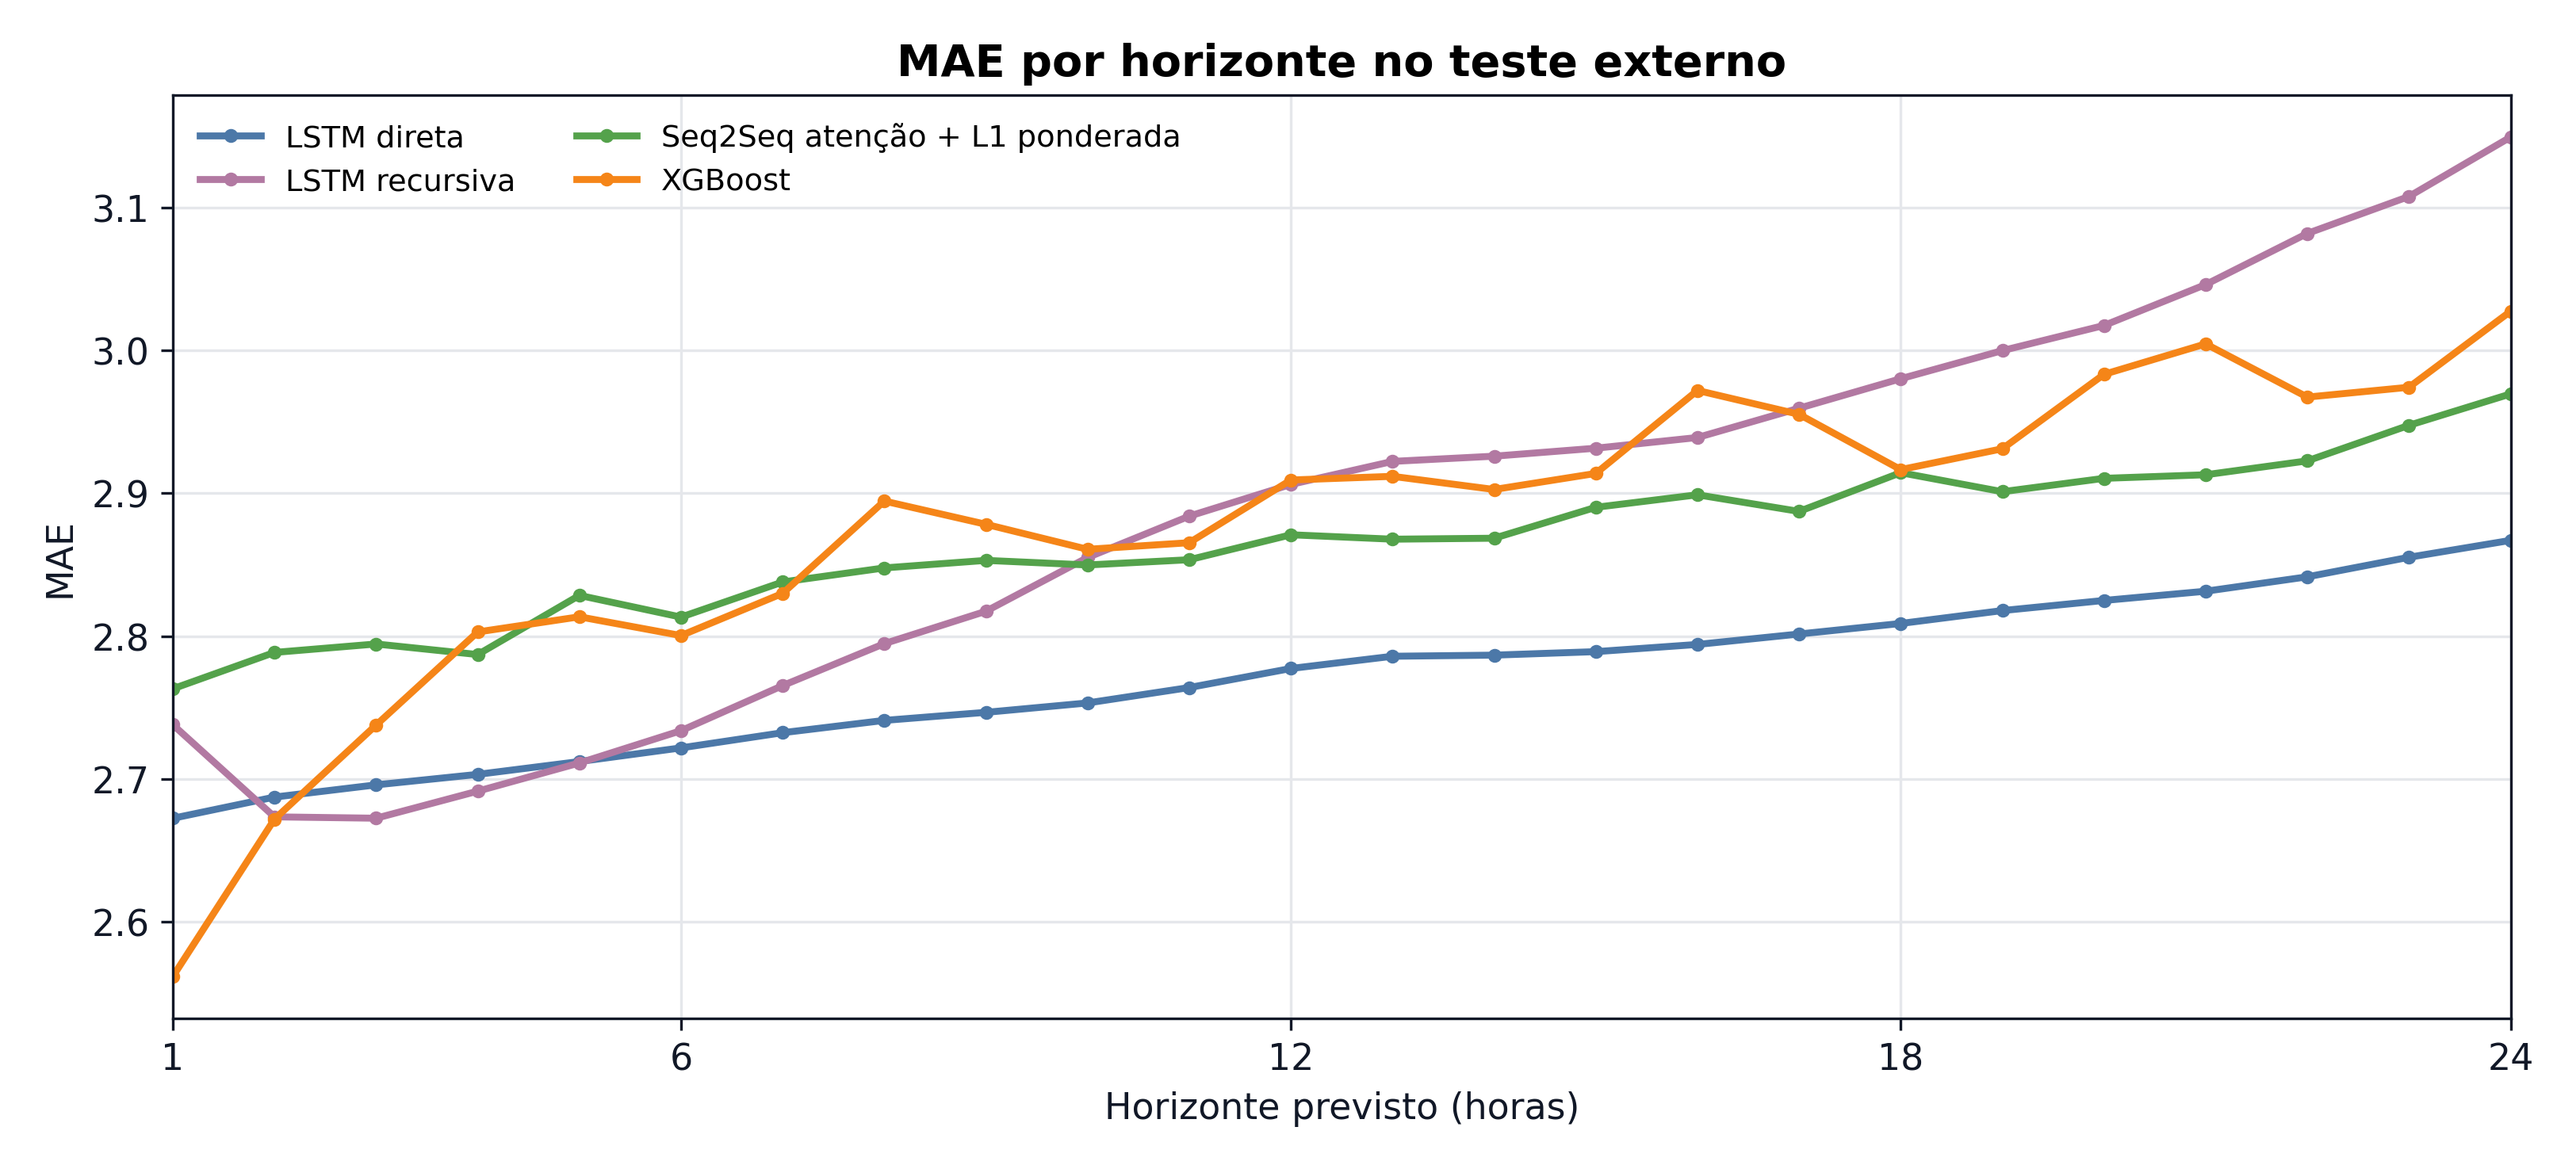
\includegraphics[width=\linewidth]{erro_por_horizonte_sapo.png}
    \caption{Evolução do MAE por horizonte no bloco final de teste para os modelos com métricas consolidadas.}
    \label{fig:erro_por_horizonte_sapo}
\end{figure}

\section{Picos, Cauda e Suavização}

A Tabela \ref{tab:cauda_sapo} mostra métricas associadas à amplitude e aos regimes altos. O desvio-padrão observado no teste é aproximadamente 5,51, e o percentil 99 (p99) resume o valor abaixo do qual se concentram 99\% das previsões ou observações. Valores da razão entre desvios-padrão abaixo de 1 indicam que a série prevista é mais suave que a série observada.

\begin{table}[htb]
    \centering
    \caption{Métricas de amplitude e cauda no teste.}
    \label{tab:cauda_sapo}
    \resizebox{\textwidth}{!}{%
    \begin{tabular}{lrrrrr}
        \toprule
        \textbf{Modelo} & \textbf{Peak35 MAE} & \textbf{p99 previsto} & \textbf{p99 observado} & \textbf{Razão desvio-padrão} & \textbf{MBE} \\
        \midrule
        LSTM direta & 13,6112 & 28,57 & 34,00 & 0,7391 & -0,1366 \\
        Seq2Seq atenção novo & \textbf{11,0815} & \textbf{32,50} & 34,00 & \textbf{0,9002} & 0,0433 \\
        XGBoost com saída múltipla & 12,2583 & 30,73 & 34,00 & 0,8506 & 0,0066 \\
        Seq2Seq atenção canônica & 14,7027 & 29,13 & 34,00 & 0,8113 & 0,0709 \\
        LSTM recursiva & 12,0392 & 30,49 & 34,00 & 0,8751 & 0,4450 \\
        Seq2Seq básico & 12,9806 & 30,65 & 34,00 & 0,8342 & -0,3855 \\
        \bottomrule
    \end{tabular}%
    }
\end{table}

Essas métricas mostram um compromisso importante. A LSTM direta vence em erro médio, mas apresenta razão entre desvios-padrão de 0,7391 e p99 previsto de 28,57, abaixo do p99 observado de 34,00. Isso sugere uma previsão mais suave e com subestimação de parte dos eventos altos. O novo Seq2Seq atenção preserva mais amplitude, com p99 previsto de 32,50, razão de desvio-padrão 0,9002 e menor Peak35 MAE. Portanto, a escolha do modelo depende do objetivo: minimizar erro médio favorece a LSTM direta; priorizar resposta a eventos altos favorece o novo Seq2Seq. A Figura \ref{fig:predito_observado_pico_sapo} reapresenta uma janela do teste em painéis separados por modelo, com escala vertical comum e interrupções nos trechos sem horários observados. Essa organização evita que as curvas disputem o mesmo eixo visual e deixa explícito que as quebras na linha observada correspondem a lacunas da própria série de teste.

\begin{figure}[htb]
    \centering
    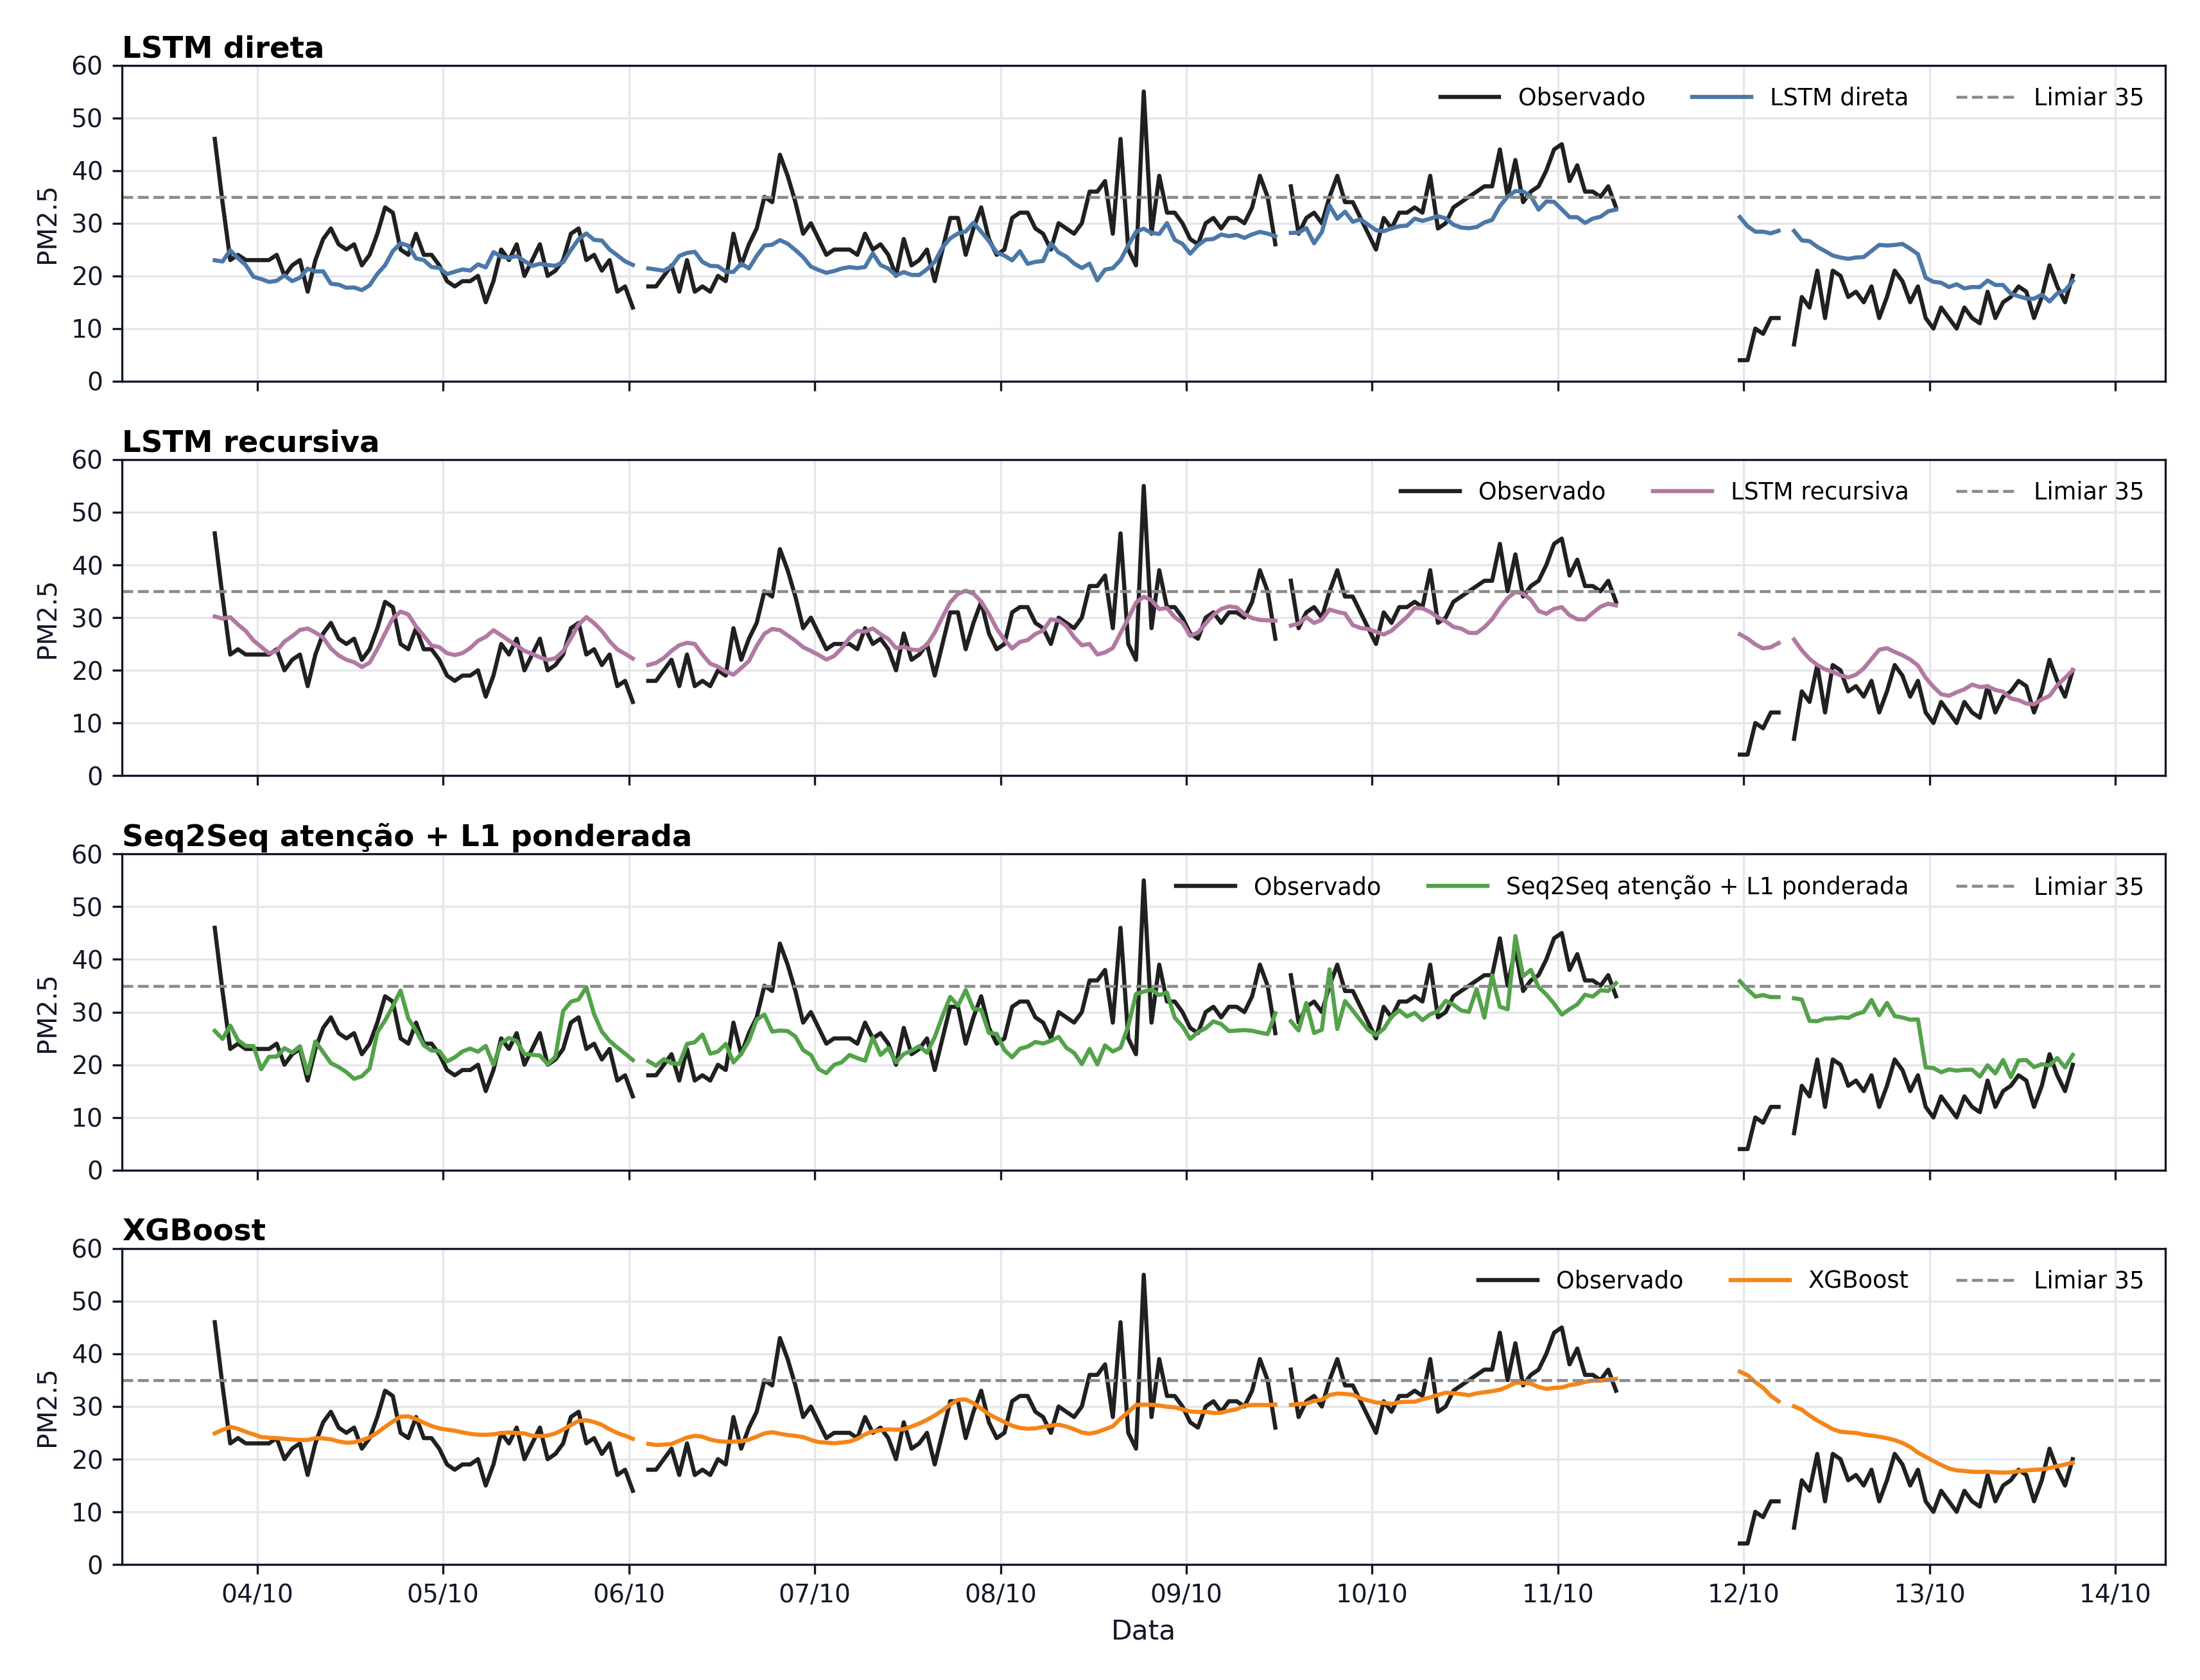
\includegraphics[width=\linewidth]{predito_observado_pico_sapo.png}
    \caption{Predições agregadas no teste em uma janela com evento de maior concentração, separadas por modelo e com interrupções nas lacunas temporais.}
    \label{fig:predito_observado_pico_sapo}
\end{figure}
\clearpage

\subsection{Análise por Evento de Pico}

Além das métricas ponto a ponto, os picos foram agregados por horário único e agrupados em eventos contínuos com PM2,5 observado \(\geq 35\). Foram encontrados 21 eventos no teste. A Tabela \ref{tab:eventos_pico_sapo} resume o erro médio dentro dos eventos, o viés médio nos eventos, a taxa de subestimação e o erro no horário do pico observado.

\begin{table}[htb]
    \centering
    \caption{Métricas por evento contínuo de pico no teste.}
    \label{tab:eventos_pico_sapo}
    \resizebox{\textwidth}{!}{%
    \begin{tabular}{lrrrr}
        \toprule
        \textbf{Modelo} & \textbf{MAE evento} & \textbf{MBE evento} & \textbf{Subestimação} & \textbf{Erro no pico observado} \\
        \midrule
        Seq2Seq atenção novo & \textbf{12,4138} & \textbf{-11,6337} & \textbf{0,8651} & \textbf{-12,7452} \\
        LSTM recursiva & 12,8186 & -12,8186 & 1,0000 & -13,6797 \\
        XGBoost com saída múltipla & 13,7253 & -13,7253 & 1,0000 & -14,7604 \\
        Persistência \(y(t)\) & 13,8803 & -13,8689 & 0,9894 & -14,9206 \\
        Sazonal \(y(t-24)\) & 14,3677 & -14,2487 & 0,9405 & -15,3809 \\
        Seq2Seq básico & 14,3725 & -14,3725 & 1,0000 & -15,5662 \\
        LSTM direta & 15,4683 & -15,4683 & 1,0000 & -16,3894 \\
        Seq2Seq atenção canônica & 15,8503 & -15,8503 & 1,0000 & -17,0143 \\
        \bottomrule
    \end{tabular}%
    }
\end{table}

A leitura por evento é mais severa que o MAE global: todos os modelos subestimam os picos, mas em graus diferentes. O novo Seq2Seq atenção tem o menor erro médio por evento, o menor viés negativo e a menor taxa de subestimação, enquanto a LSTM direta, apesar de vencer no erro global, é uma das mais conservadoras nos eventos altos. Essa evidência explicita o compromisso entre erro médio e resposta a episódios de maior concentração.

\section{Novo Seq2Seq com Atenção}

A atenção canônica com Huber não foi o melhor caminho durante o desenvolvimento, mas as ablações do Seq2Seq produziram uma variante mais forte para o contrato final. A nova configuração mantém o codificador-decodificador com atenção, usa perda ponderada por regime, remove o \textit{input feeding}, reinicia o estado do decodificador por horizonte, agrupa a atenção em \textit{buckets} de defasagem e adiciona uma perda auxiliar leve para eventos. A análise de janela indicou que 48 horas continuam sendo o melhor compromisso para essa variante: janelas de 72, 96 e 168 horas não melhoraram o MAE nem os picos.

\begin{table}[htb]
    \centering
    \caption{Novo Seq2Seq atenção no protocolo final.}
    \label{tab:novo_seq2seq}
    \resizebox{\textwidth}{!}{%
    \begin{tabular}{lrrrrr}
        \toprule
        \textbf{Variante} & \textbf{MAE} & \textbf{RMSE} & \textbf{\(R^2\)} & \textbf{Peak35 MAE} & \textbf{p99 previsto} \\
        \midrule
        Seed 42 & 2,8132 & 3,8799 & 0,5039 & 11,0815 & 32,50 \\
        Média com múltiplas sementes & 2,8218 & 3,8989 & 0,4989 & 11,5855 & 31,90 \\
        Desvio com múltiplas sementes & 0,0220 & 0,0574 & 0,0147 & 0,3771 & 0,56 \\
        \bottomrule
    \end{tabular}%
    }
\end{table}

O novo Seq2Seq substitui a variante antiga com \texttt{weighted\_l1} como representante principal da família Seq2Seq. Na semente canônica, o MAE caiu de 2,8658 para 2,8132 e o Peak35 MAE caiu de 12,3697 para 11,0815 em relação ao Seq2Seq ponderado anterior. Ainda assim, a LSTM direta permanece melhor em MAE global. A interpretação mais defensável é que o novo Seq2Seq não vence a comparação por erro médio, mas oferece o melhor compromisso entre erro agregado e preservação de picos.

\section{Ablação PM10 Causal}

A Tabela \ref{tab:ablation_pm10_causal} compara o contrato final contra duas remoções de informação: manter PM10 apenas no histórico, sem substitutos causais no decodificador, e remover PM10 completamente, deixando PM2,5 e atributos temporais. Os hiperparâmetros foram mantidos fixos a partir da seleção \textit{walk-forward}; essas ablações não fizeram nova otimização de hiperparâmetros (HPO) e foram avaliadas no mesmo bloco final de teste.

\begin{table}[htb]
    \centering
    \caption{Ablação de PM10 causal no contrato final.}
    \label{tab:ablation_pm10_causal}
    \resizebox{\textwidth}{!}{%
    \begin{tabular}{llrrrr}
        \toprule
        \textbf{Modelo} & \textbf{Contrato} & \textbf{MAE} & \textbf{\(\Delta\) MAE} & \textbf{RMSE} & \textbf{\(R^2\)} \\
        \midrule
        LSTM direta & PM10 causal completo & \textbf{2,7713} & 0,0000 & \textbf{3,8346} & \textbf{0,5154} \\
        LSTM direta & PM10 histórico sem substituto no decodificador & 2,8575 & +0,0862 & 3,9678 & 0,4812 \\
        LSTM direta & PM2,5 + tempo apenas & 2,8456 & +0,0743 & 3,9569 & 0,4840 \\
        XGBoost & PM10 causal completo & \textbf{2,8786} & 0,0000 & \textbf{3,9793} & \textbf{0,4781} \\
        XGBoost & PM10 histórico sem substituto no decodificador & 2,8873 & +0,0088 & 4,0063 & 0,4710 \\
        XGBoost & PM2,5 + tempo apenas & 2,8956 & +0,0170 & 4,0194 & 0,4676 \\
        \bottomrule
    \end{tabular}%
    }
\end{table}

A ablação confirma que os substitutos causais de PM10 foram uma decisão central, sobretudo para a LSTM direta: remover esses atributos aumentou o MAE em 0,0862, e remover PM10 completamente aumentou o MAE em 0,0743. No XGBoost, o ganho global foi menor, mas ainda consistente em MAE, RMSE e \(R^2\). Assim, o papel de PM10 causal deve ser apresentado como contribuição metodológica do contrato de dados, não apenas como detalhe de engenharia de atributos.

\section{Limite Informacional com Variáveis Futuras}

Após a ablação causal de PM10, foi executado um diagnóstico adicional com Seq2Seq atenção para responder a uma pergunta diferente: quanto do erro restante parece vir de informação futura ausente, e não apenas de arquitetura ou hiperparâmetros? Para isso, foi usado um cenário \textit{oracle future auxiliary}, no qual o decodificador recebe PM10 e partículas totais em suspensão (PTS) observados no próprio horizonte futuro. Esse cenário não representa um uso causal de previsão e não deve ser tratado como candidato a modelo final, mas funciona como limite superior informacional sob a mesma estação e tarefa.

Na estação Sapo, a tentativa de usar um conjunto mais amplo de variáveis mostrou uma limitação prática: entre as variáveis auxiliares avaliadas, PM10 e PTS foram as únicas com observações úteis de forma consistente; variáveis meteorológicas e gases estavam ausentes ou esparsos demais no recorte analisado. A Tabela \ref{tab:oracle_future_aux_sapo} resume os resultados diagnósticos.

\begin{table}[htb]
    \centering
    \caption{Diagnóstico \textit{oracle future auxiliary} no Seq2Seq atenção em Sapo.}
    \label{tab:oracle_future_aux_sapo}
    \resizebox{\textwidth}{!}{%
    \begin{tabular}{lrrrr}
        \toprule
        \textbf{Contrato diagnóstico} & \textbf{MAE} & \textbf{RMSE} & \textbf{\(R^2\)} & \textbf{Peak35 MAE} \\
        \midrule
        PM10 causal no decodificador & 2,7777 & 3,9131 & 0,4954 & 10,2406 \\
        PM10 + PTS causal no decodificador & 2,8758 & 3,9949 & 0,4741 & 10,5980 \\
        PM10 futuro real no decodificador (\textit{oracle}) & \textbf{2,4201} & 3,2659 & 0,6485 & 7,9835 \\
        PM10 + PTS futuro real no decodificador (\textit{oracle}) & 2,4223 & \textbf{3,2654} & \textbf{0,6486} & \textbf{7,1718} \\
        \bottomrule
    \end{tabular}%
    }
\end{table}

O ganho do \textit{oracle} é grande e ajuda a interpretar o problema. Em relação ao controle causal com PM10 e PTS, o uso de variáveis futuras reais reduziu o MAE de 2,8758 para 2,4223 e elevou o \(R^2\) de 0,4741 para 0,6486. A melhoria em picos também foi clara: o Peak35 MAE caiu de 10,5980 para 7,1718. Esse resultado mostra que existe informação relevante no futuro de variáveis auxiliares, especialmente em PM10, que o contrato causal não disponibiliza no instante da previsão.

Ao mesmo tempo, o próprio \textit{oracle} impõe uma leitura conservadora: mesmo com PM10 e PTS futuros reais, o \(R^2\) ficou em torno de 0,65, ainda distante de 1. Portanto, a distância até um \(R^2\) quase perfeito não parece ser apenas consequência de HPO insuficiente ou de uma arquitetura Seq2Seq subótima. Parte relevante da variância horária de PM2,5 em Sapo provavelmente depende de fatores não observados no contrato atual, como meteorologia local, estabilidade e mistura atmosférica, transporte espacial, emissões, ressuspensão e episódios súbitos.

\section{Seq2Seq Multi-Alvo com Variáveis Auxiliares}

Também foi testada uma adaptação do Seq2Seq atenção para prever PM2,5 como alvo principal e, durante o treinamento, prever PM10 e PTS futuros como tarefas auxiliares. A hipótese era que a aprendizagem conjunta poderia induzir uma representação interna mais sensível à dinâmica dos poluentes correlacionados, sem usar variáveis futuras reais no decodificador.

\begin{table}[htb]
    \centering
    \caption{Experimentos Seq2Seq multi-alvo com PM10 e PTS como tarefas auxiliares.}
    \label{tab:seq2seq_multialvo_sapo}
    \resizebox{\textwidth}{!}{%
    \begin{tabular}{lrrrr}
        \toprule
        \textbf{Variante diagnóstica} & \textbf{MAE} & \textbf{RMSE} & \textbf{\(R^2\)} & \textbf{Peak35 MAE} \\
        \midrule
        Seq2Seq causal PM10 + PTS, sem multi-alvo & 2,8758 & 3,9949 & 0,4741 & \textbf{10,5980} \\
        Multi-alvo, peso auxiliar 0,03 & 2,7997 & 4,0045 & 0,4715 & 14,5285 \\
        Multi-alvo, peso auxiliar 0,08 & 2,8876 & 4,1483 & 0,4329 & 10,5677 \\
        Multi-alvo, dimensão 128 e peso auxiliar 0,12 & \textbf{2,7689} & \textbf{3,9373} & \textbf{0,4891} & 11,3975 \\
        \bottomrule
    \end{tabular}%
    }
\end{table}

O melhor multi-alvo reduziu o MAE em relação ao controle causal com PM10 e PTS, de 2,8758 para 2,7689, e elevou o \(R^2\) de 0,4741 para 0,4891. Esse é um indício positivo de que a tarefa auxiliar pode regularizar a representação do Seq2Seq. Porém, o ganho não reproduziu o salto observado no \textit{oracle} e ainda piorou a métrica de pico em relação ao controle causal. Em termos práticos, aprender PM10 e PTS futuros não equivale a conhecer PM10 e PTS futuros.

Esses dois diagnósticos convergem para a mesma interpretação. A arquitetura pode extrair algum ganho adicional, mas o principal gargalo para \(R^2\) muito alto está na informação disponível. Sem variáveis meteorológicas e espaciais observadas de forma confiável, e sem acesso causal ao futuro dos poluentes auxiliares, o modelo tende a suavizar a variância horária e subestimar parte dos picos.

\section{Interpretação da Atenção}

Os diagnósticos anteriores dos pesos de atenção foram mantidos como evidência auxiliar, mas não são usados como argumento principal para a nova comparação final. Nas variantes avaliadas, os pesos médios de atenção não formaram um seletor temporal concentrado nem uma explicação direta da previsão. Essa cautela é coerente com a crítica de \citeonline{jain2019attention}: pesos de atenção podem ajudar a inspecionar o modelo, mas não devem ser tratados automaticamente como explicação completa da decisão.

Na rodada final, o melhor comportamento do novo Seq2Seq aparece de forma mais clara nas métricas de erro, amplitude e eventos do que na interpretação isolada da atenção. Portanto, a leitura adotada no TCC é pragmática: a atenção faz parte da arquitetura vencedora dentro da família Seq2Seq, mas o ganho observado parece depender da combinação entre contrato causal de variáveis, janela de 48 horas, desenho do decodificador, perda ponderada e seleção por ablações. Não há evidência suficiente para afirmar que o modelo aprendeu uma regra temporal simples baseada apenas em uma defasagem específica.

\section{Ablações Auxiliares e Resultados Negativos}

As ablações internas do Seq2Seq tiveram papel importante no desenvolvimento do protocolo, mas nem todas pertencem ao mesmo escopo comparável da tabela principal. Estratégias como Luong \textit{dot/general/local}, atenção temporal de múltiplas cabeças (\textit{multi-head}), portões (\textit{gates}), atenção por grupos, atenção guiada (\textit{guided attention}), DA-RNN, viés de recência (\textit{recency bias}) e variantes de \textit{scheduled sampling} foram úteis para testar hipóteses, mas não produziram ganho determinístico suficiente para alterar o vencedor global atual.

O principal achado dessas ablações não é que atenção seja irrelevante em qualquer cenário, mas que, neste conjunto de dados e sob este contrato, mudanças no contrato de dados, no uso causal de PM10 e na função de perda tiveram efeito mais claro que modificações internas sofisticadas no mecanismo de atenção. O resultado negativo também é informativo: arquiteturas mais complexas não compensam automaticamente problemas de dados, suavização ou objetivo de treinamento desalinhado com picos.

A comparação fixa inicial Sapo 70/15/15, executada sem otimização de hiperparâmetros (HPO) e com outro conjunto de variáveis, deve ser lida como etapa histórica. Ela ajudou a organizar a comparação inicial entre quatro modelos de aprendizado profundo e XGBoost, mas não é a fonte da conclusão final. A conclusão atual se baseia no protocolo final com PM10 causal, HPO \textit{walk-forward}, avaliação com múltiplas sementes dos modelos selecionados e teste no mesmo conjunto final.

\section{Ameaças à Validade}

Há limitações importantes. Primeiro, o eixo principal usa uma estação, Sapo, o que limita a generalização para outras estações e regiões. Segundo, o \textit{walk-forward} foi usado para HPO dentro dos 85\% anteriores ao teste, mas o teste final continua sendo um único bloco cronológico reservado; isso preserva o cenário temporal, mas ainda não equivale a repetir todo o estudo em múltiplas estações ou períodos independentes. Terceiro, os modelos neurais apresentam sensibilidade à semente aleatória, embora a análise com múltiplas sementes tenha reduzido a incerteza sobre a classificação por MAE. Quarto, o HPO \textit{walk-forward} do XGBoost foi limitado a quatro tentativas completas por custo computacional. Quinto, eventos de alta concentração são raros, o que torna métricas de picos instáveis e dependentes de poucos episódios.

Mesmo com essas limitações, o protocolo atual permite uma conclusão mais defensável que a narrativa anterior: no conjunto final de Sapo, a LSTM direta venceu em erro médio; o XGBoost permaneceu uma referência forte baseada em árvores sobre atributos derivados das janelas temporais; e o novo Seq2Seq atenção ficou competitivo, preservando mais amplitude e melhorando o comportamento em cauda, sem superar a LSTM direta no resultado global.

% cap_conclusao.tex
\chapter{Conclusão}
\label{chap:conclusao}

Este trabalho se propôs a desenvolver e avaliar rigorosamente uma série de modelos de aprendizado profundo para a previsão probabilística de curto prazo da concentração de material particulado PM2.5. Utilizando dados das estações de Ibirité, MG, foi realizada uma análise comparativa que demonstrou a evolução do desempenho preditivo com o aumento da complexidade arquitetônica.

A metodologia empregada, que incluiu o uso do modelo SAITS para imputação de dados, a otimização sistemática de hiperparâmetros com Optuna e a validação robusta com a técnica \textit{walk-forward}, garantiu a confiabilidade dos resultados. A principal contribuição deste estudo reside na demonstração empírica de que arquiteturas Encoder-Decoder, especialmente quando aprimoradas com mecanismos de atenção e técnicas como \textit{Scheduled Sampling}, superam significativamente modelos LSTM de base para esta tarefa.

O modelo final, um Encoder-Decoder com Atenção e \textit{Scheduled Sampling}, não apenas alcançou as melhores métricas de acurácia (MAE de 2.767), mas também forneceu previsões probabilísticas valiosas, quantificando a incerteza associada. A análise dos intervalos de confiança e dos pesos de atenção confirmou que o modelo aprendeu padrões temporais complexos e a modular sua confiança de acordo com a volatilidade dos dados.

\section{Limitações}
Apesar dos resultados promissores, o estudo possui algumas limitações. Primeiramente, a análise foi restrita a duas estações de monitoramento. A inclusão de mais estações poderia validar a generalização espacial do modelo. Em segundo lugar, o conjunto de dados, embora extenso temporalmente, não incluiu variáveis que poderiam enriquecer o contexto, como dados de tráfego veicular, focos de queimada ou informações de uso do solo, que poderiam aprimorar ainda mais as previsões. Por fim, a otimização de hiperparâmetros, embora sistemática, é um processo computacionalmente intensivo, o que limitou o espaço de busca explorado.

\section{Trabalhos Futuros}
Com base nas conclusões e limitações deste trabalho, diversas direções para pesquisas futuras podem ser exploradas:
\begin{itemize}
    \item \textbf{Modelos Espaço-Temporais:} Incorporar a relação espacial entre as estações utilizando Redes Neurais de Grafos (GNNs) em conjunto com LSTMs para capturar como a poluição se propaga entre diferentes locais.
    \item \textbf{Arquiteturas Baseadas em Transformers:} Avaliar arquiteturas mais recentes, como o Transformer puro ou variantes otimizadas para séries temporais (e.g., Informer, Autoformer), que podem capturar dependências de longo prazo de forma ainda mais eficiente que a atenção em RNNs.
    \item \textbf{Análise de Incerteza Aprimorada:} Explorar métodos mais sofisticados para estimar a incerteza, como o uso de Redes Neurais Bayesianas ou a técnica de \textit{Monte Carlo Dropout}.
    \item \textbf{Implantação e Validação Operacional:} Implementar o melhor modelo desenvolvido em um sistema de previsão em tempo real para validar seu desempenho em um ambiente operacional e fornecer alertas de qualidade do ar à população.
\end{itemize}

Em suma, este trabalho estabelece uma base sólida e uma metodologia robusta para a previsão de PM2.5 na região estudada, abrindo caminho para futuras inovações que possam contribuir ainda mais para a gestão da qualidade do ar e a proteção da saúde pública.


% =========================================================================
% ELEMENTOS PÓS-TEXTUAIS
% =========================================================================
\singlespacing
\bibliographystyle{tex/config/abntex2-alf}
\bibliography{referencias}

\end{document}